\PassOptionsToPackage{protrusion=true,expansion=false}{microtype}
\documentclass[bachelorthesis]{fer}
\usepackage{amsmath}
\numberwithin{equation}{chapter}
\usepackage{booktabs}
\usepackage{longtable}
\usepackage{array}
\usepackage{multirow}
\usepackage{calc}
\usepackage{etoolbox}
\usepackage{footnotehyper}
\makesavenoteenv{longtable}
\usepackage{float}
\usepackage{placeins}
\usepackage{makecell}
\usepackage{tabularx}
\usepackage{adjustbox}
\usepackage{ragged2e}
\usepackage{fvextra}
\usepackage{upquote}
\usepackage{microtype}
\usepackage{xurl}
\graphicspath{{./}}
\setcounter{tocdepth}{2}
\setcounter{secnumdepth}{2}
\emergencystretch=3em
\sloppy

% Pandoc compatibility helpers
\providecommand{\tightlist}{%
    \setlength{\itemsep}{0pt}\setlength{\parskip}{0pt}}
\providecommand{\pandocbounded}[1]{#1}
\newcommand{\passthrough}[1]{#1}

\newcommand{\FormulaNotationWith}[2]{%
    \vspace{-0.6em}
    \noindent\hspace*{1.2em}%
    \begin{minipage}{0.90\textwidth}
        \footnotesize
        #1
        \vspace{0.2em}
        \begin{list}{\(\bullet\)}{
            \setlength{\leftmargin}{1.4em}
            \setlength{\labelwidth}{0.8em}
            \setlength{\labelsep}{0.5em}
            \setlength{\itemsep}{0.05em}
            \setlength{\parsep}{0pt}
            \setlength{\topsep}{0.25em}
            \setlength{\partopsep}{0pt}
        }
            #2
        \end{list}
    \end{minipage}
    \par
    \vspace{0.8em}

}
\newcommand{\FormulaNotation}[1]{\FormulaNotationWith{where:}{#1}}


\title{Extending OSTrack with GRU-Based Memory Tokens for Visual Object Tracking}
\author{Illia Rotan}
\date{June 2026}
\naslov{Extending OSTrack with GRU-Based Memory Tokens for Visual Object Tracking}
\autor{Illia Rotan}
\datum{June 2026}
\mjestoEN{Zagreb}
\mjestoHR{Zagreb}
\brojrada{}
\mentor{}
\PDFTitle{Extending OSTrack with GRU-Based Memory Tokens for Visual Object Tracking}
\PDFAuthor{Illia Rotan}

\begin{document}
    \maketitle
    \frontmatter
    \tableofcontents
    \mainmatter

    \chapter*{Introduction}
    \addcontentsline{toc}{chapter}{Introduction}

    Modern visual object tracking relies heavily on matching an initial target template to a current search region. While transformer-based architectures have achieved remarkable success in this spatial matching task, they typically process frames independently, lacking an explicit mechanism to accumulate temporal information over the course of a video. Consequently, these models struggle when the target undergoes severe deformation, occlusion, or long-term appearance changes.

    This thesis investigates a memory extension of OSTrack, a state-of-the-art one-stream transformer tracker, MemOSTrack. OSTrack serves as a strong baseline because it jointly processes template and search tokens in a single transformer backbone. The thesis proposes the extantion of the original template-search token sequence with explicit recurrent memory tokens. These memory tokens are continuously updated through self-attention within the Vision Transformer and a Gated Recurrent Unit (GRU) mechanism. This update combines temporal information from previous frames with layer-wise memory refinement, granting the tracker an explicit recurrent state while preserving the core structure of the baseline.

    The scope of this work extends beyond architectural modifications to address the challenges of training a recurrent model built on a strong baseline. Because independent frame pairs are insufficient for learning temporal dynamics, the training pipeline was substantially restructured to use ordered video sequences and inference-like dynamic search cropping. By generating subsequent search crops from the model's own predictions rather than ground-truth annotations, the training conditions closely mirror real-world inference, forcing the model to learn how to recover from tracking drift. Furthermore, to prevent the network from bypassing the newly added memory pathway, explicit and implicit supervision strategies were explored. Auxiliary memory loss heads were designed to make the memory tokens predictive, while template blurring was introduced as a regularization strategy to weaken the network's over-reliance on the clean initial template.

    Additionaly, while Single-Object Tracking (SOT) is utilized as a rigorous test framework for this research—providing well-established datasets, metrics, and baselines—the core contributions of this work are not strictly limited to tracking. The proposed integration of recurrent memory tokens, layer-wise GRU updates, and dynamic sequence training provides a robust foundation that can be adapted for broader video processing tasks requiring efficient, long-term temporal modeling in Vision Transformers.

    The main contributions of this thesis are:

    \begin{itemize}
        \tightlist
        \item
        introduction of recurrent memory tokens into the OSTrack ViT backbone;
        \item
        implementation of a two-stage GRU memory update;
        \item
        rewriting of the training sampler for ordered video sequences;
        \item
        implementation of inference-like dynamic search cropping;
        \item
        exploration of memory loss heads and template blurring;
        \item
        experimental comparison with CE-enabled OSTrack baselines at 256 and 384 search
        resolutions.
    \end{itemize}


    \chapter{Background and Related Work}\label{background-and-related-work}


    \section{Single-object tracking}\label{single-object-tracking}

    Single-Object Tracking (SOT) is fundamentally a sequential computer vision problem. In the first frame of a video, a target is identified by a bounding box. In all subsequent frames, the tracker must predict the target's location without receiving any additional manual annotation. This strict initialization distinguishes tracking from ordinary object detection: identifying the class of the object is insufficient, as the tracker must follow a specific instance. If several visually similar objects are present in the scene, the correct output is the original target, not merely any object of the same category.

    \emph{Given frames \(I_1, I_2, \ldots, I_T\) and the initial box \(B_1\), a tracker predicts boxes \(\hat{B}_t\) for \(t > 1\).}

    Based on how they process this sequence, trackers can be divided into two categories. A stateless \textbf{memory-free tracker} can be written purely as a function of the initial template and the current search region, treating each frame independently. In contrast, a \textbf{recurrent tracker} additionally utilizes a hidden state carried forward from previous frames to accumulate temporal context. This distinction is central to this thesis, as MemOSTrack explicitly transitions a stateless baseline (OSTrack) into a recurrent tracker by introducing memory tokens into the backbone.

    Early tracking methods were mainly based on hand-crafted appearance and motion models, including mean-shift tracking [1], optical flow-based methods [2][16], particle filters [3], and template matching approaches [4]. These methods were often efficient and conceptually simple, but they struggled under large appearance changes, occlusion, background clutter, and scale variation. Around the early 2010s, discriminative correlation filter trackers became one of the dominant families in visual tracking. Methods such as MOSSE [5], CSK [6], KCF [7], and DSST [8] learned online filters that could localize the target efficiently in the frequency domain, while DSST also introduced a separate scale estimation mechanism. Later, more advanced correlation-filter trackers such as ECO [9] improved robustness by using more compact model updates and stronger feature representations. This period is commonly treated as the correlation-filter era of SOT, before deep Siamese and transformer-based trackers became the dominant direction.

    Despite these algorithmic advancements, tracking remains an inherently difficult task because the visual appearance of the target is rarely fixed. The target may rotate, deform, change illumination, become blurred by motion, or be partly hidden. Furthermore, the camera itself may move, producing large apparent target displacements between frames. A successful tracking method must therefore balance stability and adaptability: it must not drift to a background distractor, yet it must adapt when the true target changes appearance. Table~\ref{tab:tracking-challenges} summarizes the most common tracking challenges encountered in SOT benchmarks.

    \begin{longtable}[]{@{}
            >{\raggedright\arraybackslash}p{(\columnwidth - 4\tabcolsep) * \real{0.1449}}
            >{\raggedright\arraybackslash}p{(\columnwidth - 4\tabcolsep) * \real{0.3623}}
            >{\raggedright\arraybackslash}p{(\columnwidth - 4\tabcolsep) * \real{0.4928}}@{}}
        \caption{Common tracking challenges.}\label{tab:tracking-challenges} \\
        \toprule\noalign{}
        \begin{minipage}[b]{\linewidth}
            \raggedright
            \textbf{Challenge}
        \end{minipage} & \begin{minipage}[b]{\linewidth}
                             \raggedright
                             \textbf{Example}
        \end{minipage} & \begin{minipage}[b]{\linewidth}
                             \raggedright
                             \textbf{Why it is difficult}
        \end{minipage} \\
        \midrule\noalign{}
        \endhead
        \bottomrule\noalign{}
        \endlastfoot
        Occlusion          & Target is partially hidden                       & The visible evidence becomes incomplete and the tracker may drift. \\
        Scale change       & Target approaches the camera                     & The size of the target box changes over time.                      \\
        Deformation        & Person, animal, or flexible object changes shape & Appearance no longer matches the initial template exactly.         \\
        Background clutter & Similar objects in the scene                     & The tracker can confuse target and distractor.                     \\
        Motion blur        & Fast motion or camera movement                   & Fine details disappear from the search crop.                       \\
        Out-of-view motion & Target leaves and returns                        & The tracker state may be corrupted during absence.                 \\
    \end{longtable}


    \section{From Siamese trackers to transformer trackers}\label{from-siamese-trackers-to-transformer-trackers}

    The state of the art in single-object tracking has largely focused on template-to-target
    matching using neural networks and modern machine learning techniques, where the tracker relies on visual cues from two image regions: a template
    crop that describes the target appearance and a search crop in which the target has to
    be localized. A major step in this direction was introduced by SiamFC [10], which
    formulated tracking as a fully convolutional Siamese matching problem between an
    exemplar image and a larger search image. Later, SiamRPN [11] extended this idea by
    combining Siamese feature extraction with a region proposal subnetwork, allowing the
    tracker to perform target classification and bounding-box regression. In these early
    Siamese trackers, the template and search images are processed by two branches with
    shared convolutional weights, after which the extracted features are compared or fused
    to estimate the target location.

    Later trackers introduced transformer-based components for richer relation modeling
    between the target and the search region. STARK [12] used an encoder-decoder
    transformer to model global spatio-temporal dependencies and to directly predict the
    target bounding box. OSTrack [13] further simplified the tracking pipeline by
    introducing a one-stream transformer framework. Instead of extracting template and
    search features independently and then applying a separate relation module, OSTrack
    jointly processes template and search tokens inside the same backbone, so that feature
    extraction and relation modeling are unified.

    All of these models share a similar high-level tracking structure. They accept a
    template crop, which represents how the target looks, and a search crop, which contains
    the region of the current frame where the target is expected to appear. The tracker then
    extracts visual features from these two inputs and estimates the target position by
    comparing, fusing, or jointly modeling the template and search representations. The main
    architectural differences lie in how these features are extracted and how the relation
    between the template and search region is modeled: earlier Siamese trackers rely mainly
    on convolution and cross-correlation, while transformer-based trackers use attention
    mechanisms to allow richer interaction between template and search features.

    It is also important to note that feature extraction in modern trackers is often based
    on pretrained backbones. These backbones are pretrained on large-scale image or video
    datasets before being adapted to tracking. Because tracking datasets
    alone are usually not sufficient for learning strong low-level and semantic visual
    features from scratch. In practice, the pretrained backbone provides general visual
    representations, while tracker training teaches the model how to use these
    representations for target localization and target-background discrimination.

    Another distinct and highly influential approach worth mentioning was introduced by DiMP [15]. Unlike standard Siamese networks that simply compare the current search region against a fixed initial template, DiMP dynamically optimizes a discriminative target model during inference. By leveraging historical sequence information, it continuously updates a classifier to distinguish the target from background distractors. While DiMP relies on an explicit optimization module rather than a transformer architecture, its success shows that incorporating sequence-level information and online adaptation can significantly improve tracking robustness.


    \section{Template and Search Crop Notation}\label{template-and-search-crop-notation}

    This thesis follows the standard template-search notation used in many modern
    single-object trackers. The \textbf{template crop} is denoted by \(T\). It is extracted from
    the first annotated frame and contains the target object we are tracking.
    It is used to provide the visual description of the object that must be tracked.

    The \textbf{search crop} at time \(t\) is denoted by \(S_t\). It is extracted from the
    current frame around the expected target location. Usually, a neural-network tracker does not process the full image
    directly.
    Instead, it receives a smaller resized crop around the expected target location.
    This location is usually estimated from the bounding-box prediction in the previous frame.

    There are two main reasons why a search crop is used instead of the whole image. First,
    it reduces computation by allowing the model to process only the region where the target
    is expected to appear. This is especially important for transformer-based trackers,
    because standard full self-attention is quadratic in the number of tokens {[}18{]}. For
    example, with \(16 \times 16\) patches, a \(256 \times 256\) search crop contains 256
    tokens, whereas a full HD frame would contain more than 8000 tokens. The corresponding
    attention matrix is therefore much smaller for the search crop than for the full image.

    Second, the search crop provides a useful spatial prior. Since the crop is usually
    centered around the previous target bounding box, it gives the tracker information about
    where the target was located in the previous frame and what its approximate scale was.
    In short-term tracking, the target is usually expected to remain near its previous
    location, so a local search region is often sufficient. The tracker then predicts the
    new target box inside this resized crop, and the prediction is converted back to the
    coordinate system of the original image.

    In many trackers, the template is cropped only at initialization and remains fixed during
    the sequence. Other trackers update or maintain an additional target representation
    during inference. FEAR {[}14{]}, for example, uses a dual-template representation for object
    model adaptation, where a dynamic template complements the initial template during
    tracking.

    In contrast, trackers such as OSTrack store only the initial template extracted from the
    first frame and do not maintain an explicit updated visual template during inference.
    This makes the tracker dependent on the initial target appearance. If the target rotates,
    deforms, changes illumination, or becomes partially occluded, the initial template may no
    longer describe the current appearance well. The proposed memory mechanism is designed to reduce this limitation.
    MemOSTrack adds latent recurrent memory tokens inside the transformer
    token sequence. These memory tokens are intended to store additional temporal cues about
    the changing target appearance.


    \section{Evaluation metrics and common benchmarks}\label{evaluation-metrics-and-common-benchmarks}

    Because single-object tracking is a widely studied problem, it has established
    benchmarks and evaluation metrics. These benchmarks make it possible to compare trackers
    under a common protocol, using the same test sequences and the same localization
    measures.

    The main benchmark used in this thesis is GOT-10k. GOT-10k is a generic object tracking
    benchmark designed to evaluate how well a tracker generalizes to unseen object classes
        {[}17{]}. It follows a one-shot tracking protocol: the target is specified by a bounding box
    in the first frame, and the tracker must localize the same object in the remaining
    frames. The test annotations are hidden, so final results are obtained through the
    official evaluation server.

    The standard localization measure used in these evaluations is intersection over union
    (IoU), also called overlap. For a predicted box and a ground-truth box, IoU is the area
    of their intersection divided by the area of their union. A value of 1 means perfect
    overlap, while a value of 0 means that the boxes do not overlap.

    \begin{equation}
        \operatorname{IoU}(B_{\text{pred}}, B_{\text{gt}})
        =
        \frac{|B_{\text{pred}} \cap B_{\text{gt}}|}
        {|B_{\text{pred}} \cup B_{\text{gt}}|}
    \end{equation}
    \FormulaNotation{
        \item \(B_{\text{pred}}\) is the predicted bounding box;
        \item \(B_{\text{gt}}\) is the ground-truth bounding box;
        \item \(\cap\) denotes the intersection of the two boxes;
        \item \(\cup\) denotes the union of the two boxes;
        \item \(|\cdot|\) denotes the area of a box region.
    }

    GOT-10k reports Average Overlap (AO), SR0.50, and SR0.75 {[}17{]}. AO is computed
    as the average IoU over all evaluated frames:

    \begin{equation}
        \operatorname{AO}
        =
        \frac{1}{N}
        \sum_{i=1}^{N}
        \operatorname{IoU}(B^{i}_{\text{pred}}, B^{i}_{\text{gt}}).
    \end{equation}
    \FormulaNotation{
        \item \(\operatorname{AO}\) is the Average Overlap score;
        \item \(N\) is the number of evaluated frames;
        \item \(i\) is the frame index;
        \item \(B^{i}_{\text{pred}}\) is the predicted bounding box for frame \(i\);
        \item \(B^{i}_{\text{gt}}\) is the ground-truth bounding box for frame \(i\);
        \item \(\operatorname{IoU}(\cdot,\cdot)\) is the intersection-over-union function defined in (1.1).
    }

    SR0.50 is the proportion of frames whose overlap is at least 0.50, while SR0.75 is the
    proportion of frames whose overlap is at least 0.75. SR0.75 is stricter and is more
    sensitive to precise localization errors. These metrics are useful together because a
    tracker may localize the target approximately while still producing less accurate
    bounding boxes.


    \section{Motivation for temporal memory}\label{motivation-for-temporal-memory}

    The motivation for adding temporal memory to a tracker comes from several limitations
    of using only the initial template and the current search crop. First, the initial
    template becomes less reliable as the video progresses. It captures the target only in
    the first frame, while the target may later rotate, deform, change illumination, change
    scale, or become temporarily occluded. The current search crop can also be unreliable:
    the object may be blurred, partly hidden, or surrounded by visually similar distractors.
    In such cases, a tracker needs a mechanism that can dynamically encode the most relevant
    appearance cues from previous frames instead of relying only on the first template.

    Second, tracking is inherently temporal, a simple example can make it clear.
    Imagine looking at a patch of grass and trying to identify a camouflaged snake,
    in that one image, the snake may be almost indistinguishable from the background,
    however, once the video starts playing, coherent movement across consecutive frames can
    make the same object visible. The object has not necessarily changed its appearance, but
    the temporal context makes it easier to separate from the background. Additionally, a memory state does not need
    to store only appearance; it can potentially
    encode motion cues, learn information about recent target movement:
    direction, speed, and stable object identity across frames. This can be useful when the
    current frame is ambiguous, because the previous trajectory and recent observations can
    provide additional evidence about where the target is likely to be.

    A simple way to use temporal information would be to provide the transformer with tokens
    from previous frames together with the current search crop. However, this quickly leads
    to a temporal token explosion. For example, if one search crop contains 256 tokens, then 20 previous search crops
    already contain 5120 tokens before adding template tokens. Even
    if previous-frame key-value representations are cached, the
    current frame must still attend to a growing set of stored tokens, increasing both memory
    usage and attention cost.

    Therefore, instead of storing all previous visual tokens, an efficient tracker requires
    a reliable mechanism for dynamically maintaining a compressed hidden state. Such a state
    should preserve useful temporal cues from previous frames while keeping computation
    bounded as the sequence length increases.


    \chapter{OSTrack Baseline}\label{ostrack-baseline}


    \section{OSTrack Tracker}\label{ostrack-tracker}

    OSTrack is a real-time single-object visual tracker introduced by Ye et al. in \emph{Joint Feature Learning and Relation
    Modeling for Tracking: A One-Stream Framework}, accepted at ECCV 2022 {[}13{]}. It is used as the baseline
    tracker in this thesis because it provides a strong transformer-based architecture while keeping the tracking pipeline relatively
    simple.

    During inference, OSTrack processes one search frame at a time. It receives a fixed template crop from the first
    annotated frame and a search crop from the current frame. The tracker localizes the target inside the search crop, and
    the predicted bounding box is then used to define the search region for the next frame.

    The main architectural idea of OSTrack is its one-stream design. Instead of extracting template and search features
    separately and then applying a separate relation module, OSTrack converts both crops into tokens and processes them
    jointly in a single Vision Transformer (ViT) backbone. As a result, feature extraction and template-search relation
    modeling
    are performed inside the same backbone. Self-attention over the combined token sequence allows template and search
    tokens to interact throughout the network, which helps the model learn target-oriented search features {[}13{]}.

    After the ViT backbone, OSTrack uses a lightweight fully convolutional prediction head. The final search tokens are
    reshaped into a two-dimensional spatial feature map and passed to this head. The head has three fully convolutional
    output branches, which predict a classification score map, a local offset map, and a normalized bounding-box size map.
    The position with the highest classification score is selected as the target position.
    The backbone is initialized from a pretrained ViT model.

    OSTrack also supports candidate elimination, which progressively removes less relevant search
    tokens to reduce computation; this mechanism is described separately in Section 2.3.


    \section{ViT Backbone}\label{vit-backbone}

    OSTrack is built on a pretrained Vision Transformer (ViT) backbone. Most of the modifications in this thesis are focused on the ViT backbone.
    ViT is a powerful image-processing architecture that has shown strong performance in
    computer vision and, with large-scale pretraining, can match or outperform state-of-the-art
    convolutional networks on several image-recognition benchmarks. ViT represents an image as a sequence of patch tokens and processes this sequence
    using transformer encoder layers {[}19{]}. In OSTrack, this structure is adapted to tracking by applying patch embedding to
    both the template crop and the search crop, and then processing the resulting tokens jointly in the same backbone {[}13{]}.

    \begin{figure}[htbp]
        \centering
        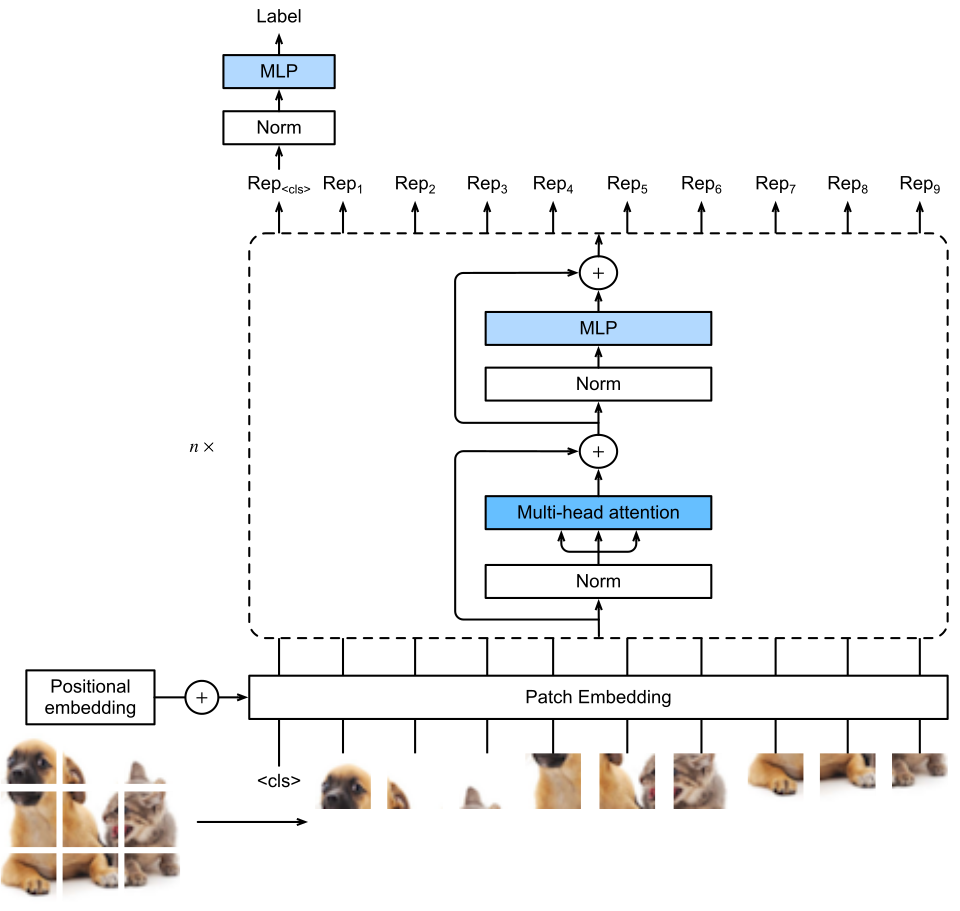
\includegraphics[width=0.65\textwidth]{vit_example.png}
        \caption{Vision Transformer architecture. Vision Transformer.svg by Zhang, Lipton, Li, and Smola, licensed under CC BY-SA 4.0, via Wikimedia Commons [22].}
        \label{fig:vit}
    \end{figure}

    During the ViT processing of an image crop \(X\), the image is first divided into non-overlapping patches:

    \begin{equation}
        \begin{aligned}
            N &= \frac{HW}{P^2},
            \qquad
            X_p = [x_1, x_2, \ldots, x_N]^\top
            \in \mathbb{R}^{N \times P^2C}.
        \end{aligned}
    \end{equation}
    \FormulaNotation{
        \item \(X \in \mathbb{R}^{H \times W \times C}\) is the input image crop;
        \item \(H\) and \(W\) are the height and width of the crop;
        \item \(C\) is the number of image channels;
        \item \(P\) is the patch size;
        \item \(N\) is the number of patches;
        \item \(x_i \in \mathbb{R}^{P^2C}\) is the flattened vector of the \(i\)-th patch;
        \item \(X_p\) is the sequence of all flattened patch vectors.
    }

    A standard ViT encoder layer applies a pre-normalized multi-head self-attention block followed by a pre-normalized per-token MLP
    block, with residual connections after both. In the CE-enabled OSTrack backbone, candidate elimination is inserted
    between the attention block and the MLP block. This gives the following \(\operatorname{ViTBackbone}\) layer update:

    \begin{align}
        U_l &=
        Z_{l-1}
        +
        \operatorname{MSA}\left(\operatorname{LN}(Z_{l-1})\right),
        \\[0.5em]
        \tilde{U}_l &=
        \begin{cases}
            \operatorname{CE}_l(U_l), & \text{if CE pruning is enabled at layer } l, \\
            U_l, & \text{otherwise},
        \end{cases}
        \\[0.5em]
        Z_l &=
        \tilde{U}_l
        +
        \operatorname{MLP}\left(\operatorname{LN}(\tilde{U}_l)\right).
    \end{align}
    \FormulaNotation{
        \item \(l\) is the transformer layer index;
        \item \(Z_{l-1}\) is the input token sequence to layer \(l\);
        \item \(U_l\) is the intermediate sequence after the attention block and residual connection;
        \item \(\tilde{U}_l\) is the token sequence after optional CE pruning;
        \item \(Z_l\) is the output token sequence of layer \(l\);
        \item \(\operatorname{LN}(\cdot)\) denotes Layer Normalization;
        \item \(\operatorname{MSA}(\cdot)\) denotes Multi-Head Self-Attention;
        \item \(\operatorname{CE}_l(\cdot)\) denotes candidate elimination at layer \(l\);
        \item \(\operatorname{MLP}(\cdot)\) denotes the feed-forward block.
    }

    Multi-head self-attention allows each token to exchange information with other tokens in the same sequence. Since OSTrack,
    template and search tokens are processed together, self-attention provides the mechanism
    through which template-search interaction occurs inside the backbone.

    Candidate elimination is specific to OSTrack and is not part of the original ViT architecture. It is only present when
    CE pruning is enabled. The detailed CE mechanism is described separately in Section 2.3.

    OSTrack applies this ViT backbone to a pair of tracking crops. Let \(T\) denote the template crop and \(S_t\) denote the
    search crop at frame \(t\). Their token sequences are denoted by \(T_0\) and \(S_{t,0}\), and the tracker processes their
    concatenation:

    \begin{equation}
        Z_{t,0}^{\mathrm{track}} = [T_0, S_{t,0}].
    \end{equation}

    After \(L\) transformer layers, the backbone output is

    \begin{equation}
        \begin{aligned}
            Z_{t,L}^{\mathrm{track}}
            &=
            \operatorname{ViTBackbone}\left(Z_{t,0}^{\mathrm{track}}\right)
            \\
            &=
            [T_L^{(t)}, S_{t,L}].
        \end{aligned}
    \end{equation}
    \FormulaNotation{
        \item \(T_0 \in \mathbb{R}^{N_T \times D}\) is the template-token sequence;
        \item \(S_{t,0} \in \mathbb{R}^{N_S \times D}\) is the search-token sequence for frame \(t\);
        \item \([\cdot,\cdot]\) denotes concatenation along the token dimension;
        \item \(L\) is the number of transformer layers;
        \item \(T_L^{(t)}\) is the processed template-token representation;
        \item \(S_{t,L}\) is the processed search-token representation.
    }

    The final search-token representation \(S_{t,L}\) is reshaped into a spatial feature map and passed to the prediction
    head.


    \section{Candidate elimination}\label{candidate-elimination}

    OSTrack introduces candidate elimination (CE) to reduce the number of search tokens processed by the transformer
    backbone. In a template-search tracker, the search crop contains both the target and many background patches. CE removes
    search tokens that are unlikely to correspond to the target, reducing computation while keeping the most relevant
    candidates [13].

    OSTrack chooses candidates using attention between the template and search tokens. After the multi-head attention
    operation in a transformer block, a representative template token is used to score the search tokens. In the standard
    setting, this representative token is the center template token, because the target is normally centered in the template
    crop. If this token is denoted by \(\phi\) and the transformer has \(M\) attention heads, the score of search token
    \(x\) is computed by averaging attention from \(\phi\) to \(x\) over all heads:

    \begin{equation}
        w_x^{\phi} = \frac{1}{M}\sum_{m=1}^{M} w_x^{\phi}(m).
    \end{equation}
    \FormulaNotation{
        \item \(w_x^{\phi}\) is the averaged attention score from the representative template token to search token \(x\);
        \item \(\phi\) is the representative template token;
        \item \(x\) is a search token;
        \item \(M\) is the number of attention heads;
        \item \(m\) is the attention-head index;
        \item \(w_x^{\phi}(m)\) is the attention score from \(\phi\) to \(x\) in head \(m\).
    }

    Search tokens with the highest scores are kept, while lower-scoring search tokens are
    removed from the sequence for later transformer layers. If \(k\) tokens are kept from
    \(n\) current search tokens, the keep ratio is:

    \begin{equation}
        k = \operatorname{round}(\rho n).
    \end{equation}
    \FormulaNotation{
        \item \(\rho\) is the keep ratio;
        \item \(k\) is the integer number of search tokens kept after pruning;
        \item \(n\) is the number of current search tokens before pruning.
    }

    The kept search-token indices can be written as:

    \begin{equation}
        I_{\text{keep}} = \operatorname{TopK}(w_x^{\phi}, k).
    \end{equation}
    \FormulaNotation{
        \item \(I_{\text{keep}}\) is the set of retained search-token indices;
        \item \(\operatorname{TopK}(\cdot,k)\) selects the \(k\) highest-scoring tokens;
        \item \(w_x^{\phi}\) is the attention-based score used for ranking search tokens.
    }

    The original order and positions of the remaining search tokens are stored. Before the
    prediction head, the kept search tokens are restored to their spatial order and the
    removed positions are zero-padded so that the spatial search feature map can be
    reconstructed {[}13{]}.

    This matters for MemOSTrack because the proposed model adds memory tokens to the OSTrack
    token sequence. In this implementation, CE is applied only to search tokens. Template
    tokens are preserved, and memory tokens are also preserved because they are recurrent
    latent states rather than spatial search candidates. Memory tokens participate in
    attention, but they are not used to score search candidates and are not removed by CE.
    Thus, candidate elimination keeps its original role of pruning search-region candidates,
    while the recurrent memory stream remains available throughout the backbone.


    \chapter{Proposed Memory-Augmented OSTrack}\label{proposed-memory-augmented-ostrack}


    \section{Memory-token design motivation}\label{memory-token-design-motivation}

    MemOSTrack extends OSTrack by adding explicit memory tokens to the transformer backbone.
    These memory tokens are inserted into the same token sequence as the template
    and search image feature embeddings, so they participate in ViT attention together with the visual
    tokens. However, unlike template and search tokens, memory tokens are latent hidden-state vectors
    rather than image patches, and they are carried across frames during tracking.

    This design allows the ViT backbone to continuously read from and refine the memory representation
    through attention. Visual tokens can interact with memory tokens while the current
    template and search features are processed, and the resulting memory representation can
    store information that may be useful in later frames.

    The architectural changes are mainly applied inside the backbone. The patch embedding
    and OSTrack prediction head are kept close to the baseline implementation, so the model
    remains an OSTrack-style tracker with an added recurrent memory stream.


    \section{Direct transformer-based memory update}\label{direct-transformer-based-memory-update}

    The first architectural variant adds memory tokens to the OSTrack backbone and lets the
    ViT layers update them directly. In this version, memory tokens are concatenated with
    the template and search tokens and are processed by the same transformer layers as the
    visual tokens. The goal is to allow memory to interact with search and template tokens through the existing attention operations.

    The ViT backbone is modified to process transformed template,
    search, and memory tokens in a single forward pass:

    \begin{equation}
    [T_{t,l}, S_{t,l}, M_{t,l}]
        =
        \operatorname{ViTLayer}_l
        \left(
        [T_{t,l-1}, S_{t,l-1}, M_{t,l-1}]
        \right).
    \end{equation}
    \FormulaNotationWith{Here:}{
        \item \(T_{t,l}\) denotes the template tokens after layer \(l\) while processing frame \(t\);
        \item \(S_{t,l}\) denotes the search tokens after layer \(l\) while processing frame \(t\);
        \item \(M_{t,l-1}\) is the memory input from the previous transformer layer in the current frame;
        \item \(M_{t,l}\) is the memory output produced directly by the ViT layer;
        \item \(\operatorname{ViTLayer}_l(\cdot)\) denotes transformer layer \(l\).
    }

    All token groups have the same embedding dimension \(D\), so they can be concatenated
    along the token dimension and processed by the same transformer block.

    For the first frame of a sequence, no previous memory state exists, so the model uses a learned initial memory state.
    After each consecutive frame is processed, the backbone returns an updated memory state in the auxiliary output,
    which is then fed back into the backbone together with the template and the next search crop when processing the next frame.


    To distinguish memory tokens from visual tokens, the model adds a learned memory-token
    type embedding to the memory tokens before they are processed by the backbone. This
    embedding shifts the memory tokens in feature space and gives the transformer a learned
    signal that allows the model to distinguish these tokens as memory states rather than image patches.

    In the CE-enabled backbone, memory tokens are intentionally excluded from
    candidate-elimination decisions. First, they are not pruned, because CE removes only
    search tokens. Second, they are excluded from the template mask used for CE scoring, so
    they do not directly influence which search tokens are kept or removed. Thus, CE pruning is decided without treating
    them as either removable candidates or
    scoring tokens, so memory tokens can influence it only indirectly through their
    participation in transformer attention.

    \begin{figure}[htbp]
        \centering
        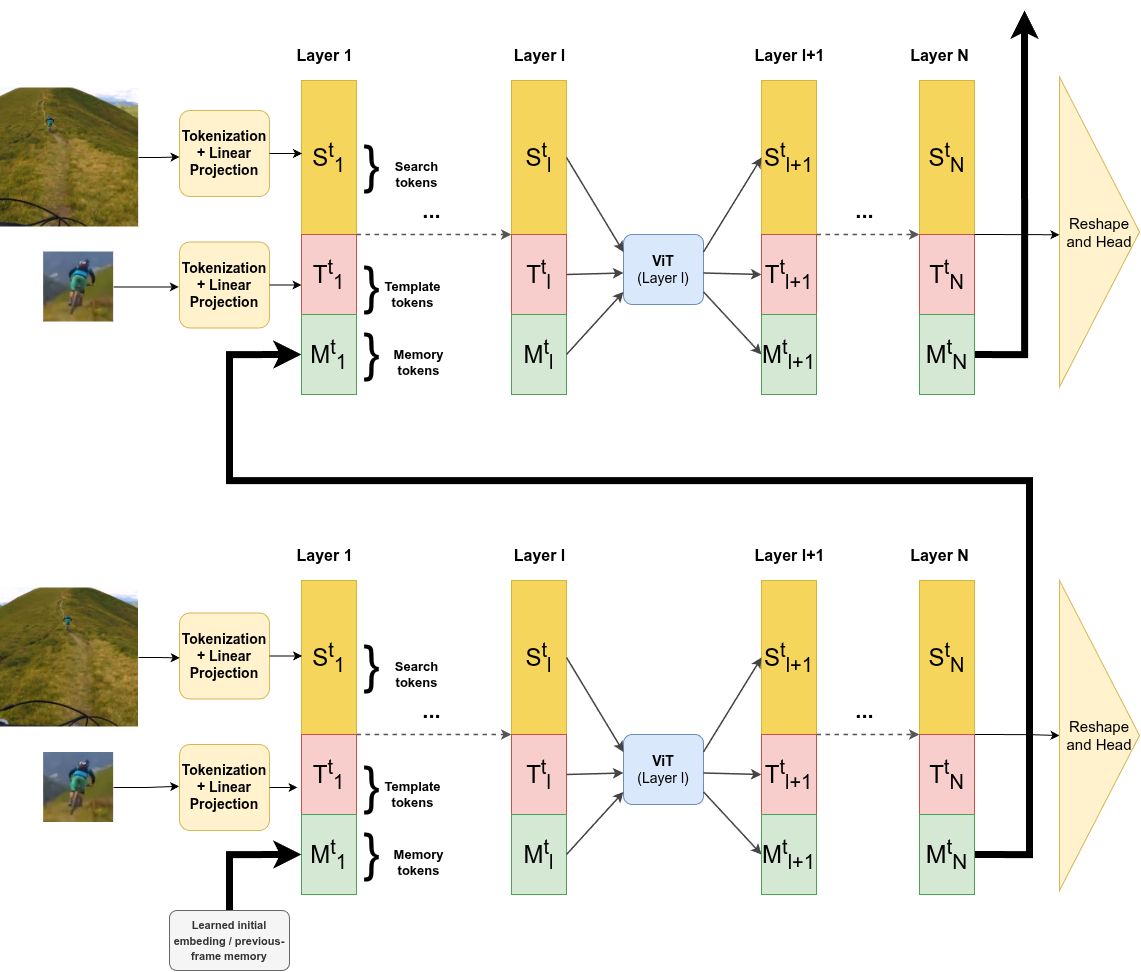
\includegraphics[width=0.9\textwidth]{memostrack_backbone_layers_no-gru.png}
        \caption{Direct transformer-based memory update. The template and search images are first converted into visual tokens by tokenization and linear projection. A learned initial memory state, or the memory state returned from the previous frame, is inserted into the transformer token sequence. Each ViT layer jointly processes template, search, and memory tokens through self-attention. The updated memory state is passed through the backbone and returned for use in the next frame, while the final visual tokens are reshaped and passed to the OSTrack prediction head.}
        \label{fig:direct-memory-update}
    \end{figure}


    \section{Limitations of direct memory update}\label{limitations-of-direct-memory-update}

    When used for long-term temporal modeling, the direct-update variant exposes two fundamental limitations.
    While the standard Vision Transformer architecture is effective for
    spatial feature extraction and template-search matching, relying on it alone for
    recurrent memory updates might is insufficient.

    The first limitation is the lack of explicit gating for memory preservation. In the direct-update variant,
    memory tokens are updated directly by the same transformer block. The attention mechanism is effective
    for deciding which template and search tokens should influence the memory representation, however, it does not provide
    a dedicated gate that controls how much of the previous memory should be kept and how much new information should be written.

    Equation~\ref{eq:vit-attention-residual} provides a residual path that can preserve information from the
    previous layer:

    \begin{equation}
        U_l =
        Z_{l-1}
        +
        \operatorname{MSA}\left(\operatorname{LN}(Z_{l-1})\right).
        \label{eq:vit-attention-residual}
    \end{equation}

    Since \(Z_{l-1}\) includes the memory tokens in the direct-update variant,
    this residual connection passes their previous layer representation forward.
    While in principle, the model can learn to produce a small attention update,
    \(\operatorname{MSA}(\operatorname{LN}(Z_{l-1}))\),
    when the memory does not need to change much, this mechanism may be weaker than an explicit update gate.
    Over long tracking sequences, repeated ungated updates may still gradually alter the memory state and make it less representative of the target.


    The second limitation is the susceptibility to gradient instability during Backpropagation Through Time due
    to an absence of temporal skip connections. In recurrent neural networks, there are often temporal skip connections
    between the memory representations of the same layer across time. However, in the direct-update design, recurrence is
    present only in the form of a feedback loop, where the last layer of the current frame is connected to the first layer
    of the next frame. This means that when unrolling the memory tokens over \(T\) frames through an \(L\)-layer backbone, the
    gradient has to travel through all layers of the backbone for each frame:

    \begin{equation}
        \frac{\partial L_T}{\partial M_1}
        \supset
        \frac{\partial L_T}{\partial M_T}
        \prod_{t=2}^{T}
        \prod_{l=1}^{L}
        \frac{\partial M_{t,l}}{\partial M_{t,l-1}} .
    \end{equation}
    \FormulaNotationWith{Here:}{
        \item \(L_T\) is the loss at frame \(T\);
        \item \(M_1\) and \(M_T\) are the memory states at the first and last frames;
        \item \(t\) is the frame index;
        \item \(l\) is the transformer layer index;
        \item \(L\) is the number of transformer layers;
        \item \(\frac{\partial M_{t,l}}{\partial M_{t,l-1}}\) represents the local Jacobian matrix at layer \(l\) of frame \(t\);
        \item \(\supset\) indicates that the expression shows one component of the full gradient path.
    }
    This expression isolates the recurrent memory path; the full training gradient also contains paths through search
    tokens,
    template tokens, the prediction head, and the backbone parameters.

    Because the search and template tokens do not propagate their hidden states across frames,
    the recurrent temporal path is carried by the memory tokens, represented here by
    \(\frac{\partial M_{t,l}}{\partial M_{t,l-1}}\).
    Suppose we have a 12-layer transformer backbone over a 20-frame sequence;
    this chain expands to 240 sequential Jacobian matrix multiplications. This deep computational graph can contribute to
    error accumulation, causing gradient vanishing or explosion. One way to
    address this issue is to add explicit temporal skip connections.

    To address both memory drift and gradient instability, a more intentional architectural design is required.
    Specifically, the architecture must decouple the \emph{proposal} of new memory from the actual \emph{update} of the memory state,
    and it must introduce explicit temporal skip connections to stabilize gradient flow. This motivates the second
    architectural variant, which replaces the direct update with a two-way gated recurrent mechanism, as detailed in the
    following section.


    \section{Two-way GRU. GRU-based memory update.}\label{variant-b-gru-based-memory-update-and-two-stage-architecture}

    To implement this controlled update, the second architectural variant introduces a Gated Recurrent Unit (GRU) mechanism
    to the memory stream. A GRU is a recurrent module that updates a hidden state using learned gates {[}20{]}. These gates
    control how much of the previous state is preserved and how much new information is accepted. This is highly suitable
    for memory tokens because the tracker must retain reliable target information while still adapting when the target
    appearance changes.

    In this version, the transformer layer does not directly produce the final memory. Instead, the transformer output is
    treated as a candidate memory representation:

    \begin{equation}
    [T_{t,l}, S_{t,l}, M'_{t,l}]
        =
        \mathrm{ViTLayer}_l([T_{t,l-1}, S_{t,l-1}, M_{t,l-1}]).
    \end{equation}
    \FormulaNotation{
        \item \(M'_{t,l}\) is the candidate memory representation proposed by the transformer layer;
        \item \(T_{t,l}\) and \(S_{t,l}\) are the template and search tokens after layer \(l\) at frame \(t\);
        \item \(M_{t,l-1}\) is the memory from the previous layer in the current frame;
        \item \(\mathrm{ViTLayer}_l(\cdot)\) denotes transformer layer \(l\).
    }

    The value \(M'_{t,l}\) is the memory suggested by attention at the current frame and layer. It is not accepted directly.
    Instead, it is passed to a two-stage GRU update. The first GRU combines the candidate memory with the memory from the
    previous frame at the same layer, creating an explicit temporal skip connection:

    \begin{equation}
        \tilde{M}_{t,l} = \mathrm{GRU}_1(M'_{t,l}, M_{t-1,l}).
    \end{equation}
    \FormulaNotation{
        \item \(\tilde{M}_{t,l}\) is the intermediate memory after temporal fusion;
        \item \(\mathrm{GRU}_1(\cdot,\cdot)\) is the first GRU update, applied independently to each memory token;
        \item \(M'_{t,l}\) is the current candidate memory and is used as the GRU input;
        \item \(M_{t-1,l}\) is the memory from the previous frame at the same layer and is used as the previous hidden state.
    }

    The second GRU combines the intermediate memory with memory from the previous
    layer in the current frame:

    \begin{equation}
        M_{t,l} = \mathrm{GRU}_2(\tilde{M}_{t,l}, M_{t,l-1}).
    \end{equation}
    \FormulaNotation{
        \item \(M_{t,l}\) is the final memory output at frame \(t\) and layer \(l\);
        \item \(\mathrm{GRU}_2(\cdot,\cdot)\) is the second GRU update, applied independently to each memory token;
        \item \(\tilde{M}_{t,l}\) is the intermediate memory after temporal fusion and is used as the GRU input;
        \item \(M_{t,l-1}\) is the memory from the previous layer in the current frame and is used as the previous hidden state.
    }

    The final output of the layer is:

    \begin{equation}
        Y_{t,l} = [T_{t,l}, S_{t,l}, M_{t,l}].
    \end{equation}
    \FormulaNotation{
        \item \(Y_{t,l}\) is the final token sequence output of layer \(l\) at frame \(t\);
        \item \([\cdot,\cdot,\cdot]\) denotes concatenation along the token dimension;
        \item \(T_{t,l}\), \(S_{t,l}\), and \(M_{t,l}\) are the template, search, and memory tokens after the layer update.
    }

    This recurrent update is used only when previous-frame memory is available. On the
    first frame, the tracker initializes memory from the learned initial memory state and
    skips the temporal GRU comparison with a previous frame.
    The first GRU can be interpreted as temporal fusion. It decides how much memory
    from frame \(t-1\) should remain when the current candidate memory is introduced.
    The second GRU can be interpreted as layer-wise fusion. It allows memory from
    the previous transformer layer to influence the final memory at the current
    layer, creating a gated depth path for memory tokens.

    \begin{figure}[htbp]
        \centering
        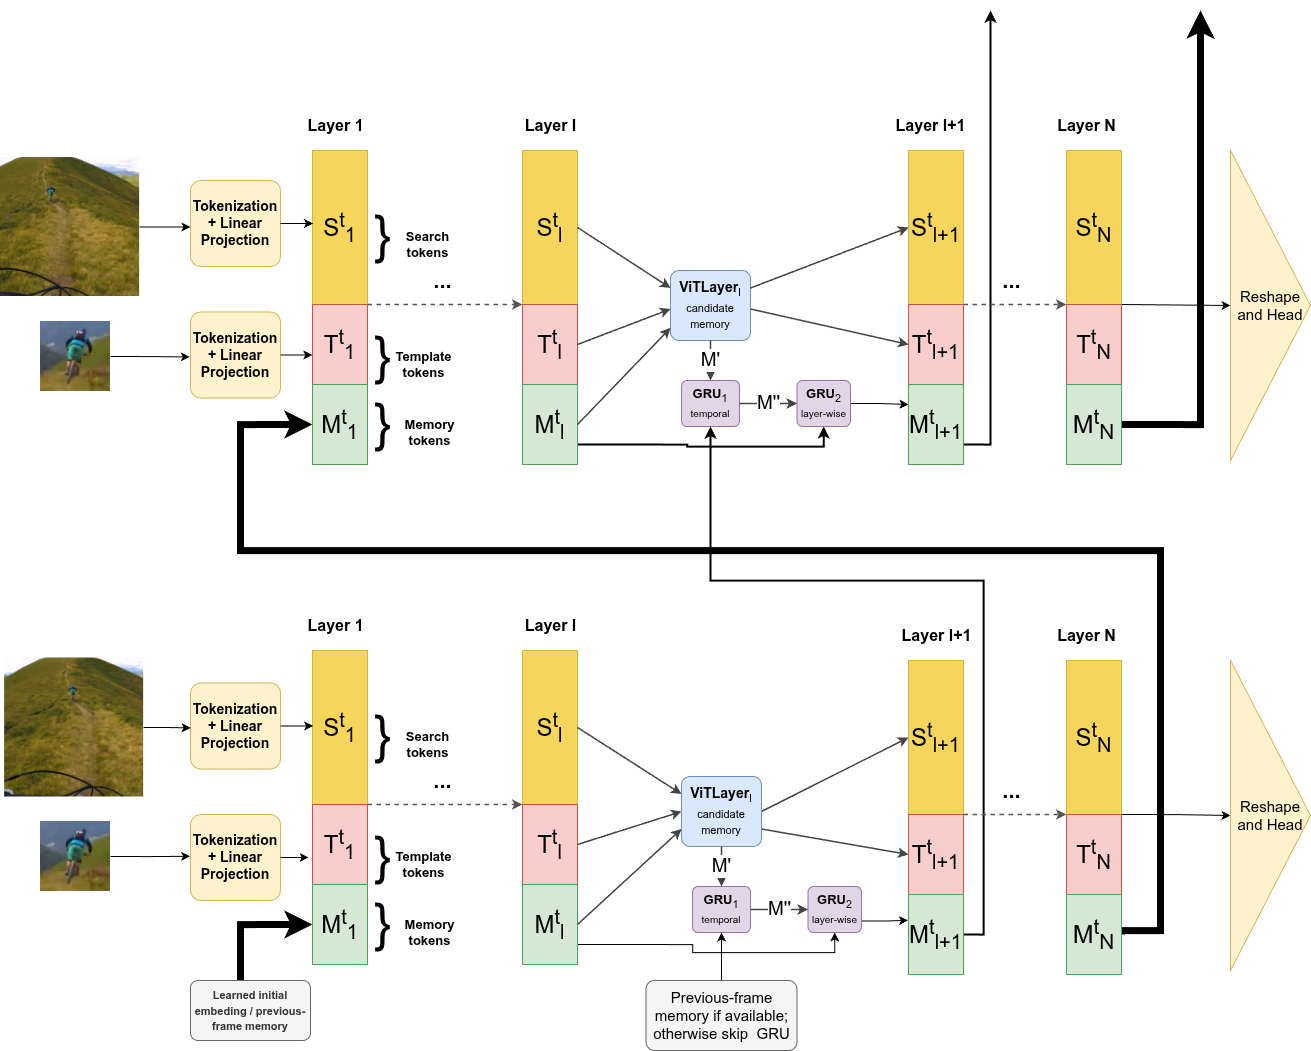
\includegraphics[width=0.9\textwidth]{memostrack_backbone_layers-gru.png}
        \caption{GRU-based memory update with temporal and depth connections inside the backbone.}
        \label{fig:gru-memory-update}
    \end{figure}

    This design was introduced in the later stage of development. The GRU update makes the memory stream explicitly recurrent and gives
    the model a learned mechanism for balancing preservation and adaptation.

    A related alternative considered during development was a three-way gated
    update. In that design, the final memory would be a weighted combination of the
    three available memory sources:

    \begin{equation}
        M_{t,l} = \alpha_1 M'_{t,l}
        + \alpha_2 M_{t-1,l}
        + \alpha_3 M_{t,l-1},
        \quad
        \alpha_1 + \alpha_2 + \alpha_3 = 1.
    \end{equation}
    \FormulaNotation{
        \item \(M_{t,l}\) is the resulting memory at frame \(t\) and layer \(l\);
        \item \(M'_{t,l}\), \(M_{t-1,l}\), and \(M_{t,l-1}\) are the candidate, previous-frame, and previous-layer memory sources;
        \item \(\alpha_1\), \(\alpha_2\), and \(\alpha_3\) are learned mixture weights;
        \item \(\alpha_1 + \alpha_2 + \alpha_3 = 1\) constrains the weights to sum to one.
    }

    Such a softmax-style gate would make the three-source structure explicit. The
    implemented version instead uses two sequential GRU updates. The GRU version is
    more recurrent in form and uses learned gates inside each update. The three-way
    gated update remains a useful future architecture to explore because it would treat all three memory
    sources symmetrically.


    \chapter{Sequence-Based and Inference-Like Training}\label{sequence-based-and-inference-like-training}


    \section{Sequence-based training for recurrent memory}\label{sequence-based-training-for-recurrent-memory}

    Standard OSTrack training is based on independent template-search pairs. A template crop
    is sampled from one frame, a search crop is sampled from another frame in the same video,
    and the model is trained to predict the target box inside the search crop:

    \begin{equation}
        \text{sample} = (T, S_t, B_t), \qquad \hat{B}_t = f(T, S_t).
    \end{equation}
    \FormulaNotationWith{Here:}{
        \item \(\text{sample}\) denotes one pair-based training sample;
        \item \(T\) is the template crop;
        \item \(S_t\) is the search crop at time \(t\);
        \item \(B_t\) is the ground-truth target box expressed in the coordinate system of the search crop;
        \item \(\hat{B}_t\) is the predicted target box at time \(t\);
        \item \(f(\cdot)\) is the tracker model.
    }
    Because the standard tracker is memory-free, processing each training sample independently is sufficient.

    However, for correct MemOSTrack training, independent pair-based training is inadequate. A recurrent memory state \(M_t\) must evolve over a continuous sequence of frames from the same video. The standard single-step horizon makes it impossible for the network to learn usefull long-term temporal dependencies. Conversely, carrying the memory state forward across randomly sampled, unrelated pairs would feed the model incorrect historical context.

    Therefore, the sampling pipeline was rewritten to return ordered search-frame sequences. In this
    causal consecutive setting, the sampled frames follow the natural temporal direction of the video. The training sample becomes:

    \begin{equation}
        \text{sample} = (T, S_1, S_2, \dots, S_N, B_1, B_2, \dots, B_N).
    \end{equation}
    \FormulaNotation{
        \item \(\text{sample}\) denotes one sequence-based training sample;
        \item \(T\) is the template crop;
        \item \(S_1, S_2, \dots, S_N\) are ordered search crops from the same video;
        \item \(B_1, B_2, \dots, B_N\) are the corresponding target boxes;
        \item \(N\) is the number of search frames in the sampled sequence.
    }

    For each frame in the sequence, the model predicts a bounding box and updates its memory state. The memory output from frame \(t-1\) becomes the input for frame \(t\). Preserving this exact temporal order provides the recurrent memory module with a meaningful path to learn across time.


    \section{Dynamic inference-like search cropping}\label{dynamic-search-cropping}

    Sequence-based sampling makes recurrent memory training possible, but it does not by
    itself remove the mismatch between training and inference. If every search crop is
    centered using the ground-truth box of the current frame, the tracker receives cleaner
    inputs than it will receive at test time. The target is usually near the center of the
    crop, and the model does not experience the consequences of its own previous prediction
    errors.

    In standard ground-truth-centered training, the search crop is generated using the ground-truth box of the current frame:

    \begin{equation}
        S_t = \operatorname{crop}(I_t, B^{gt}_t).
    \end{equation}
    \FormulaNotation{
        \item \(S_t\) is the search crop at time \(t\);
        \item \(I_t\) is the full image at time \(t\);
        \item \(B^{gt}_t\) is the ground-truth target box at time \(t\).
    }

    To simulate imperfect localization, standard training applies artificial random jitter to this ground-truth box. However, even with this jitter, the inputs remain fundamentally disconnected from the model's actual performance. Because every crop is anchored to the true target location, the model never experiences the compounding prediction errors that occur during real tracking.

    During inference, the tracker does not know the current ground-truth target location.
    The next search crop must be generated from the previous prediction:


    \begin{equation}
        S_t = \operatorname{crop}(I_t, \hat{B}_{t-1}).
    \end{equation}
    \FormulaNotation{
        \item \(\hat{B}_{t-1}\) is the predicted bounding box from the previous frame.
    }

    This prediction-centered cropping allows localization errors to accumulate. A poor prediction in one frame will shift the target away from the center in the next frame, potentially leading to complete tracking failure. This difference is especially critical for a recurrent tracker, as an inaccurate crop will directly corrupt the memory state passed to subsequent frames.


    To close this gap, the final training pipeline introduces inference-like dynamic search cropping. The tracker is initialized using the first-frame ground truth, but all subsequent crops in the sequence are generated dynamically from the model's predictions. At each step, the model processes the template, the current search crop, and the previous memory state to predict the new target box and update the memory:

    \begin{equation}
        \begin{aligned}
            S_t &= \operatorname{crop}(I_t, \hat{B}_{t-1}), \\
            \hat{B}_t, M_t &= f(T, S_t, M_{t-1}).
        \end{aligned}
    \end{equation}
    \FormulaNotation{
        \item \(S_t\) is the search crop generated dynamically for frame \(t\);
        \item \(\hat{B}_{t-1}\) is the previous predicted box used to center and scale the crop;
        \item \(\hat{B}_t\) is the predicted box at time \(t\);
        \item \(M_t\) is the updated memory state at time \(t\);
        \item \(T\) is the template crop;
        \item \(M_{t-1}\) is the memory state from the previous frame;
        \item \(f(\cdot)\) is the MemOSTrack model.
    }

    This dynamic loop intentionally makes training more difficult. With ground-truth-centered crops, the model sees clean examples even if its previous predictions would have been inaccurate. With dynamic cropping, an early localization error can move the next crop away from the target center, which can cause the target to appear partially outside the crop. However, this difficulty is necessary to close the gap between training and inference and provides two major benefits. First, it allows the model to properly learn motion cues, as the displacement of the target within the crop directly reflects its actual movement relative to the previous frame. Second, it give the model an opporunity to learn how to recover from its own mistakes; by experiencing the consequences of poor predictions during training, the tracker learns to re-center the target and correct tracking drift before it leads to complete failure.

    Because dynamic cropping makes optimization more difficult, the final training pipeline used a curriculum training strategy.
    During the first 40 epochs, search crops were centered using ground-truth target boxes. After this warm-up phase,
    inference-like dynamic cropping was enabled, so each next crop was generated from the model's previous prediction. This
    allowed the model to first learn stable localization before being exposed to prediction drift.


    \section{Truncated Backpropagation Through Time in the training loop}\label{truncated-backpropagation-through-time-in-the-training-loop}

    The introduction of memory tokens transforms the tracker into a recurrent model, necessitating careful management of
    error backpropagation across temporal iterations. Allowing gradients to flow through an entire video sequence is both
    computationally expensive and highly demanding on GPU memory. Additionally, unrolling the computational graph over long
    sequences amplifies the risk of gradient instability, such as vanishing or exploding gradients. A standard approach to
    address this is truncating backpropagation through time. In the provided implementation, the model periodically
    detaches the memory state from the computation graph after a fixed number of frames (specifically, 8 frames during
    training). This truncation limits how far the gradients can propagate backward in time, balancing the need to learn
    temporal dependencies with computational feasibility and training stability.


    \chapter{Auxiliary Memory Supervision}\label{auxiliary-memory-supervision}


    \section{Auxiliary Loss Concept}\label{auxiliary-loss-concept}

    Adding memory tokens to a strong model does not guarantee that the model will actually use them.
    OSTrack already possesses a powerful template-search matching pathway. Because the tracker can often solve the
    training task using template and search tokens alone, the newly introduced memory tokens may receive
    weak gradients. This creates the risk that the memory tokens can collapse to an uninformative representation
    or are entirely ignored by the prediction head.

    This is a common issue when adding auxiliary modules to strong neural networks: the optimization process often follows the dominant low-loss pathway. If the template is clean and the search crop is well-centered, that pathway may rely entirely on the original OSTrack features, leaving the memory branch with little to no effect on the final prediction.

    To address this, this thesis explored auxiliary memory supervision. The goal was to force the memory tokens to encode representations that are directly useful for prediction, rather than remaining passive elements within the token sequence.


    \section{Sampled Discriminative Filter Loss}\label{sampled-discriminative-filter-loss}

    The first auxiliary loss was designed to explicitly force the memory tokens to encode spatial representations capable of localizing the target. To achieve this, an auxiliary memory head was introduced to the architecture. This lightweight multi-layer perceptron takes only the recurrent memory tokens as input and projects them into a spatial convolutional filter. Rather than allowing the memory tokens to remain abstract, this approach evaluates their discriminative power by testing how well this predicted filter can localize the target across the video sequence.

    Let \(f_t\) denote the memory filter predicted by the memory head at frame \(t\). To evaluate this filter, a random subset
    of frames, denoted by the index set \(\mathcal{S}_t\), is sampled from the current training sequence. For each sampled
    frame \(j \in \mathcal{S}_t\), the filter \(f_t\) is applied to the corresponding search region feature map \(x_j\) via
    cross-correlation to produce a spatial response map:

    \begin{equation}
        s_{t,j} = x_j * f_t.
    \end{equation}
    \FormulaNotation{
        \item \(s_{t,j}\) is the spatial response map produced by filter \(f_t\) on frame \(j\);
        \item \(x_j\) is the search-region feature map for sampled frame \(j\);
        \item \(f_t\) is the memory filter predicted at frame \(t\);
        \item \(*\) denotes cross-correlation.
    }

    The objective is to minimize the discrepancy between this predicted response map and the ground-truth Gaussian target heatmap \(y_j\). The loss for the filter at frame \(t\) is formulated as the mean squared error over the sampled subset, combined with an \(L_2\) regularization penalty on the filter weights:

    \begin{equation}
        \begin{aligned}
            L_t &= \frac{1}{|\mathcal{S}_t|}
            \sum_{j \in \mathcal{S}_t}
            \lVert x_j * f_t - y_j \rVert_2^2
            + \lambda \lVert f_t \rVert_2^2.
        \end{aligned}
    \end{equation}
    \FormulaNotationWith{Here:}{
        \item \(L_t\) is the auxiliary loss for the filter predicted at frame \(t\);
        \item \(\mathcal{S}_t\) is the sampled subset of frames used to evaluate filter \(f_t\);
        \item \(|\mathcal{S}_t|\) is the number of sampled frames in that subset;
        \item \(j\) is the sampled-frame index;
        \item \(x_j\) is the search-region feature map for frame \(j\);
        \item \(f_t\) is the memory filter predicted at frame \(t\);
        \item \(y_j\) is the ground-truth Gaussian target heatmap for frame \(j\);
        \item \(\lambda\) is a hyperparameter controlling the strength of the weight regularization.
    }
    The total auxiliary loss is the average of \(L_t\) across all frames in the sequence that
    produce a memory filter.

    A critical design choice in this algorithm is the treatment of the search features \(x_j\). During the loss computation,
    these features are explicitly detached from the computational graph. If the search features were not detached, gradients
    from this auxiliary loss would flow backward through them and into the ViT backbone for the sampled frames. That would
    force the backbone to modify its general visual representations to accommodate the memory loss. By detaching the
    features, the optimization gradients are forced to propagate exclusively backward through the predicted filter \(f_t\),
    the auxiliary memory head, and into the recurrent memory tokens. This ensures that the loss strictly supervises the
    memory pathway without inadvertently altering the primary feature extractor.

    The primary strength of this loss is that it evaluates the memory representation in a direct, tracking-oriented manner:
    the memory state must generate a filter that yields a high response at the target location and a low response on the
    background, even when applied to frames from different temporal steps.

    However, this approach presents two significant limitations. First, because the supervision relies on a randomly sampled subset of frames (\(\mathcal{S}_t\)), the training signal can exhibit high variance and noise. Second, the computational complexity scales poorly. Evaluating every predicted filter against every other frame in a sequence of length \(T\) requires \(O(T^2)\) cross-correlation operations. While random sampling reduces this to \(O(T \cdot |\mathcal{S}_t|)\), it remains computationally heavy. These limitations motivated the development of a more efficient, sequence-level approach, detailed in the following section.


    \section{DiMP Target-Match Loss}\label{dimp-target-match-loss}

    The second auxiliary loss is the DiMP-style target-match loss. Instead of directly testing every predicted memory
    filter on sampled features from previous frames, this loss first constructs a stronger sequence-level target filter and
    then trains each predicted memory filter to match it.

    This idea is inspired by DiMP {[}15{]}, where tracking is formulated as learning a target-specific discriminative model from
    training samples. DiMP showed that online target model prediction can use both target and background information,
    instead of only matching a target template {[}15{]}.

    The proposed DiMP-style target-match loss is not a reimplementation of the full DiMP tracker. Instead, it borrows the
    idea of fitting a discriminative target filter from a sequence of search features. The fitted filter is then used as a
    detached pseudo-label for the memory branch. This differs from original DiMP, where the optimized filter is the actual
    target classifier used for tracking. The simplification is intentional: the goal is not to replace OSTrack's prediction
    head, but to provide direct supervision that encourages the added memory tokens to encode information useful for target
    discrimination.

    To construct the pseudo-label, the method first collects all available detached search features, \(x_1, \dots, x_T\), and
    their corresponding ground-truth heatmaps, \(y_1, \dots, y_T\). An initial filter is formed by taking the mean of the
    detached memory filters predicted by the auxiliary memory head across the sequence. A sequence-level target
    filter, \(f^*\), is then fitted by minimizing the following least-squares objective:

    \begin{equation}
        \begin{aligned}
            L(f) &= \operatorname{mean}\left(\lVert x * f - y \rVert_2^2\right)
            + \lambda \operatorname{mean}\left(\lVert f \rVert_2^2\right).
        \end{aligned}
    \end{equation}
    \FormulaNotationWith{Here:}{
        \item \(L(f)\) is the least-squares objective for fitting a target filter;
        \item \(f\) is the candidate discriminative filter being optimized;
        \item \(x\) denotes the collected detached search features;
        \item \(y\) denotes the corresponding ground-truth heatmaps;
        \item \(\lambda\) is the regularization strength;
        \item \(\operatorname{mean}(\cdot)\) denotes averaging over the evaluated samples and spatial locations;
        \item \(f^*\) is the filter that best matches the whole training sequence under this least-squares objective.
    }
    The implementation
    solves this using a steepest-descent solver with an analytic step length.

    After computing the target filter, the memory filters predicted by the memory head are trained to match it. The final
    auxiliary loss is the mean squared difference between each predicted filter and the optimized target filter:

    \begin{equation}
        L_{\text{match}} = w_{\text{match}} \frac{1}{M} \sum_i \lVert f_i - f^* \rVert_2^2.
    \end{equation}
    \FormulaNotation{
        \item \(L_{\text{match}}\) is the target-match auxiliary loss;
        \item \(w_{\text{match}}\) is \texttt{FILTER\_MATCH\_WEIGHT};
        \item \(M\) is the number of predicted memory filters;
        \item \(i\) indexes the predicted memory filters;
        \item \(f_i\) is the predicted memory filter from frame \(i\);
        \item \(f^*\) is the optimized sequence-level target filter.
    }

    This loss has several advantages over the sampled discriminative filter loss described in Section 5.2. It provides the
    memory branch with a more stable target, because \(f^*\) is estimated from the full sequence rather than a small random
    sample. It trades the computation of cross-correlation on every frame during loss evaluation for the upfront
    optimization of a single sequence-level correlation filter. While running the inner optimization solver is a heavier
    operation, it ultimately becomes faster than the quadratic complexity emerging from recomputing cross-correlations
    between every predicted filter and all previous frames. Furthermore, the loss encourages temporal consistency, as all
    memory filters are pulled toward the same sequence-level target model.

    Despite its computational advantages, the target-match loss introduces notable trade-offs. Primarily, it relies heavily
    on the quality of the pseudo-label. If the inner optimization yields an inaccurate filter \(f^*\)---such as during heavy
    occlusion---the memory tokens are penalized for imitating a flawed model. Furthermore, this supervision is highly
    prescriptive. By forcing memory tokens to project into a spatial correlation filter, it restricts the transformer from
    freely encoding other potentially useful temporal cues, such as motion or abstract relations.

    Because of the architectural complexity and constrained nature of explicit auxiliary losses, this thesis also explored a complementary, implicit regularization strategy: Template Blurring, detailed in the following section.


    \section{Template Blurring}\label{template-blurring}

    To complement the explicit auxiliary losses, this thesis also explores template blurring as an implicit
    memory-supervision
    strategy. Because the baseline OSTrack architecture already possesses a highly effective template-search matching
    pathway, the model can often solve the training task without utilizing the newly introduced memory tokens. Template
    blurring artificially degrades the reliability of the initial template and may encourage the tracker to use the recurrent
    memory tokens as an alternative source of target appearance information.

    Let \(z\) denote the original template and \(\tilde{z}\) the corrupted template. Two corruption modes were considered: a
    blur
    mode (\(\tilde{z} = \text{Blur}(z)\)) using repeated average pooling, and a zero-masking mode (\(\tilde{z} = 0\)). The blur
    mode is less aggressive, removing high-frequency appearance details while preserving coarse structural cues. However,
    because the model might still recover useful information from a blurred template, zero-masking was also introduced. By
    completely removing the template's visual features, zero-masking creates maximum pressure on the network to extract and
    utilize the historical target information stored in the memory tokens.

    During training, template corruption is applied randomly to a subset of frames within the sampled sequence. A
    critical design choice is that the first few search frames are strictly excluded from corruption. This allows
    the tracker to process clean frames initially and build a reliable memory state before template corruption is
    introduced.
    Consequently, this mechanism is only applied to sufficiently long training sequences to ensure a proper balance between
    clean and corrupted inputs.

    Template corruption is strictly a training-time regularization technique; during inference, the tracker always receives
    the clean initial template.

    The primary advantage of template blurring is its architectural simplicity. It requires no additional loss heads, inner
    optimization solvers, or pseudo-labels. The tracker is optimized entirely through the standard localization losses,
    while the input corruption naturally shifts the network's internal reliance toward the memory stream. Furthermore,
    because it alters the actual tracking pathway rather than just an intermediate representation, improved performance on
    corrupted frames suggests that the memory tokens may provide target appearance cues.

    As a result, template blurring serves as a controlled training condition that weakens the dominant template
    matching, offering a simple and implicit alternative to explicit auxiliary losses.


    \chapter{Experimental Setup}\label{experimental-setup}


    \section{Dataset and protocol}\label{dataset-and-protocol}

    The experiments are performed on the GOT-10k dataset {[}17{]}, a generic object tracking benchmark comprising over 10,000 video segments and 1.5 million labeled bounding boxes. Because the test set annotations are withheld, final evaluation is performed by submitting predictions to the official benchmark server. To ensure a fair comparison, training is conducted exclusively on the GOT-10k training split, without incorporating any additional tracking datasets.


    \section{Model configuration}\label{model-configuration}

    As a baseline, the OSTrack model with a 256-pixel search crop and Candidate Elimination (CE) pruning was chosen.
    Following the original OSTrack configuration, the ViT backbone is initialized from an MAE-pretrained checkpoint {[}21{]}.

    The proposed MemOSTrack configuration builds upon this baseline with the following specifications. The model processes
    a \(128 \times 128\) pixel template crop (64 template tokens) and a \(256 \times 256\) pixel search crop
    (256 search tokens). To this visual sequence, 64 memory tokens are added, bringing the initial sequence length
    to 384 tokens. The memory tokens are updated inside the transformer backbone via the proposed two-stage GRU recurrent mechanism.

    The training pipeline employs a causal consecutive sequence sampler under a two-stage curriculum. To stabilize early
    optimization, the first 40 epochs utilize ground-truth-centered crops with random jitter over 20-frame rollouts.
    After this warm-up stage, inference-like dynamic cropping is fully enabled, and the rollout length is reduced to 15 frames.


    \section{Evaluation protocol}\label{evaluation-protocol}

    The tracker is evaluated on the GOT-10k test set using Average Overlap (AO), Success Rate at 0.50 (SR0.50), and Success
    Rate at 0.75 (SR0.75), as defined in Section 1.4.

    The comparison is made against reported OSTrack-256 + CE and OSTrack-384 + CE
    baselines. The 256-pixel baseline is the closest architectural comparison because it uses the
    identical template and search crop resolution, while the 384-pixel baseline is included as a stronger, high-resolution reference.

    Because the proposed MemOSTrack model introduces several changes simultaneously, the
    final result should not be interpreted as identifying a single cause. A comprehensive ablation study separating the individual effects of memory tokens, dynamic cropping, GRU configurations, and auxiliary loss weights is left for future work.


    \chapter{Results and Discussion}\label{results-and-discussion}


    \section{Quantitative Results}\label{quantitative-results}

    The final measured result for MemOSTrack-256 + CE is shown in Table~\ref{tab:got10k-results}. The model achieved AO 0.729, SR0.50 0.823, and SR0.75 0.693. The reported OSTrack-256 + CE baseline achieves AO 0.710, SR0.50 0.804, and SR0.75 0.682. The stronger high-resolution OSTrack-384 + CE baseline achieves AO 0.737, SR0.50 0.832, and SR0.75 0.708 [13].

    \begin{longtable}[]{@{}lrrr@{}}
        \caption{Final quantitative comparison on GOT-10k.}\label{tab:got10k-results} \\
        \toprule\noalign{}
        \textbf{Method}     & \textbf{AO} & \textbf{SR0.50} & \textbf{SR0.75} \\
        \midrule\noalign{}
        \endhead
        \bottomrule\noalign{}
        \endlastfoot
        OSTrack-256 + CE    & 0.710       & 0.804           & 0.682           \\
        MemOSTrack-256 + CE & 0.729       & 0.823           & 0.693           \\
        OSTrack-384 + CE    & 0.737       & 0.832           & 0.708           \\
    \end{longtable}

    The final MemOSTrack configuration improves upon the reported same-resolution OSTrack-256 + CE baseline across all three
    metrics, achieving gains of +0.019 in AO, +0.019 in SR0.50, and +0.011 in SR0.75. This shows that the complete MemOSTrack training pipeline can improve tracking accuracy at the same search resolution. However, because the final model combines several changes: memory tokens, GRU-based updates, sequence-based training, dynamic cropping, and auxiliary supervision strategies, a full ablation study would be required to separate the contribution of each component.

    The result remains slightly below the reported OSTrack-384 + CE baseline. This is expected, because the 384-resolution baseline processes a larger template and search region, giving it access to finer spatial detail. MemOSTrack-256 closes part of the gap to this stronger high-resolution model, but it does not surpass it.

    To contextualize the accuracy comparison, Table~\ref{tab:speed-comparison} reports the measured inference speed on an NVIDIA RTX A6000 GPU. The table also includes the initial number of input tokens processed by the backbone. With a patch size of (16 \times 16), OSTrack-256 uses 64 template tokens and 256 search tokens, resulting in 320 initial tokens. MemOSTrack-256 adds 64 recurrent memory tokens, increasing the initial sequence length to 384 tokens. In contrast, OSTrack-384 uses a larger template and search region, resulting in 720 initial tokens.

    \begin{longtable}[]{@{}lrr@{}}
        \caption{Input-token budget and inference speed on NVIDIA RTX A6000.}\label{tab:speed-comparison} \
        \toprule\noalign{}
        \textbf{Method} & \textbf{Initial tokens} & \textbf{FPS} \
        \midrule\noalign{}
        \endhead
        \bottomrule\noalign{}
        \endlastfoot
        OSTrack-256 + CE    & 320 & 131.46 \
        MemOSTrack-256 + CE & 384 & 97.73 \
        OSTrack-384 + CE    & 720 & 72.85 \
    \end{longtable}

    The measured speed confirms that the added recurrent memory is not computationally free. MemOSTrack-256 + CE runs at 97.73 FPS, compared with 131.46 FPS for the direct OSTrack-256 + CE baseline. This slowdown is expected because the memory tokens increase the sequence length processed by the transformer backbone and because the model also performs recurrent memory updates.

    At the same time, MemOSTrack-256 + CE remains substantially faster than the high-resolution OSTrack-384 + CE baseline, which runs at 72.85 FPS. This is important because ViT-based trackers are sensitive to sequence length, especially in the self-attention layers where the cost grows quadratically with the number of tokens. Although runtime is not determined by token count alone, the measured FPS supports the intended trade-off: MemOSTrack-256 improves over the same-resolution OSTrack-256 baseline while remaining more efficient than simply increasing the tracking resolution to 384. The remaining accuracy gap to OSTrack-384 + CE is therefore consistent with the larger spatial token budget and higher computational cost of the high-resolution model.


    \section{Training Dynamics}\label{training-dynamics}

    To understand how the model adapts during training, the learning dynamics were analyzed throughout the training process.
    Figure~\ref{fig:train-metrics} and Figure~\ref{fig:validation-metrics} illustrate the training and validation metrics, respectively, which reflect the
    distinct phases of the training strategy.

    \begin{figure}[htbp]
        \centering
        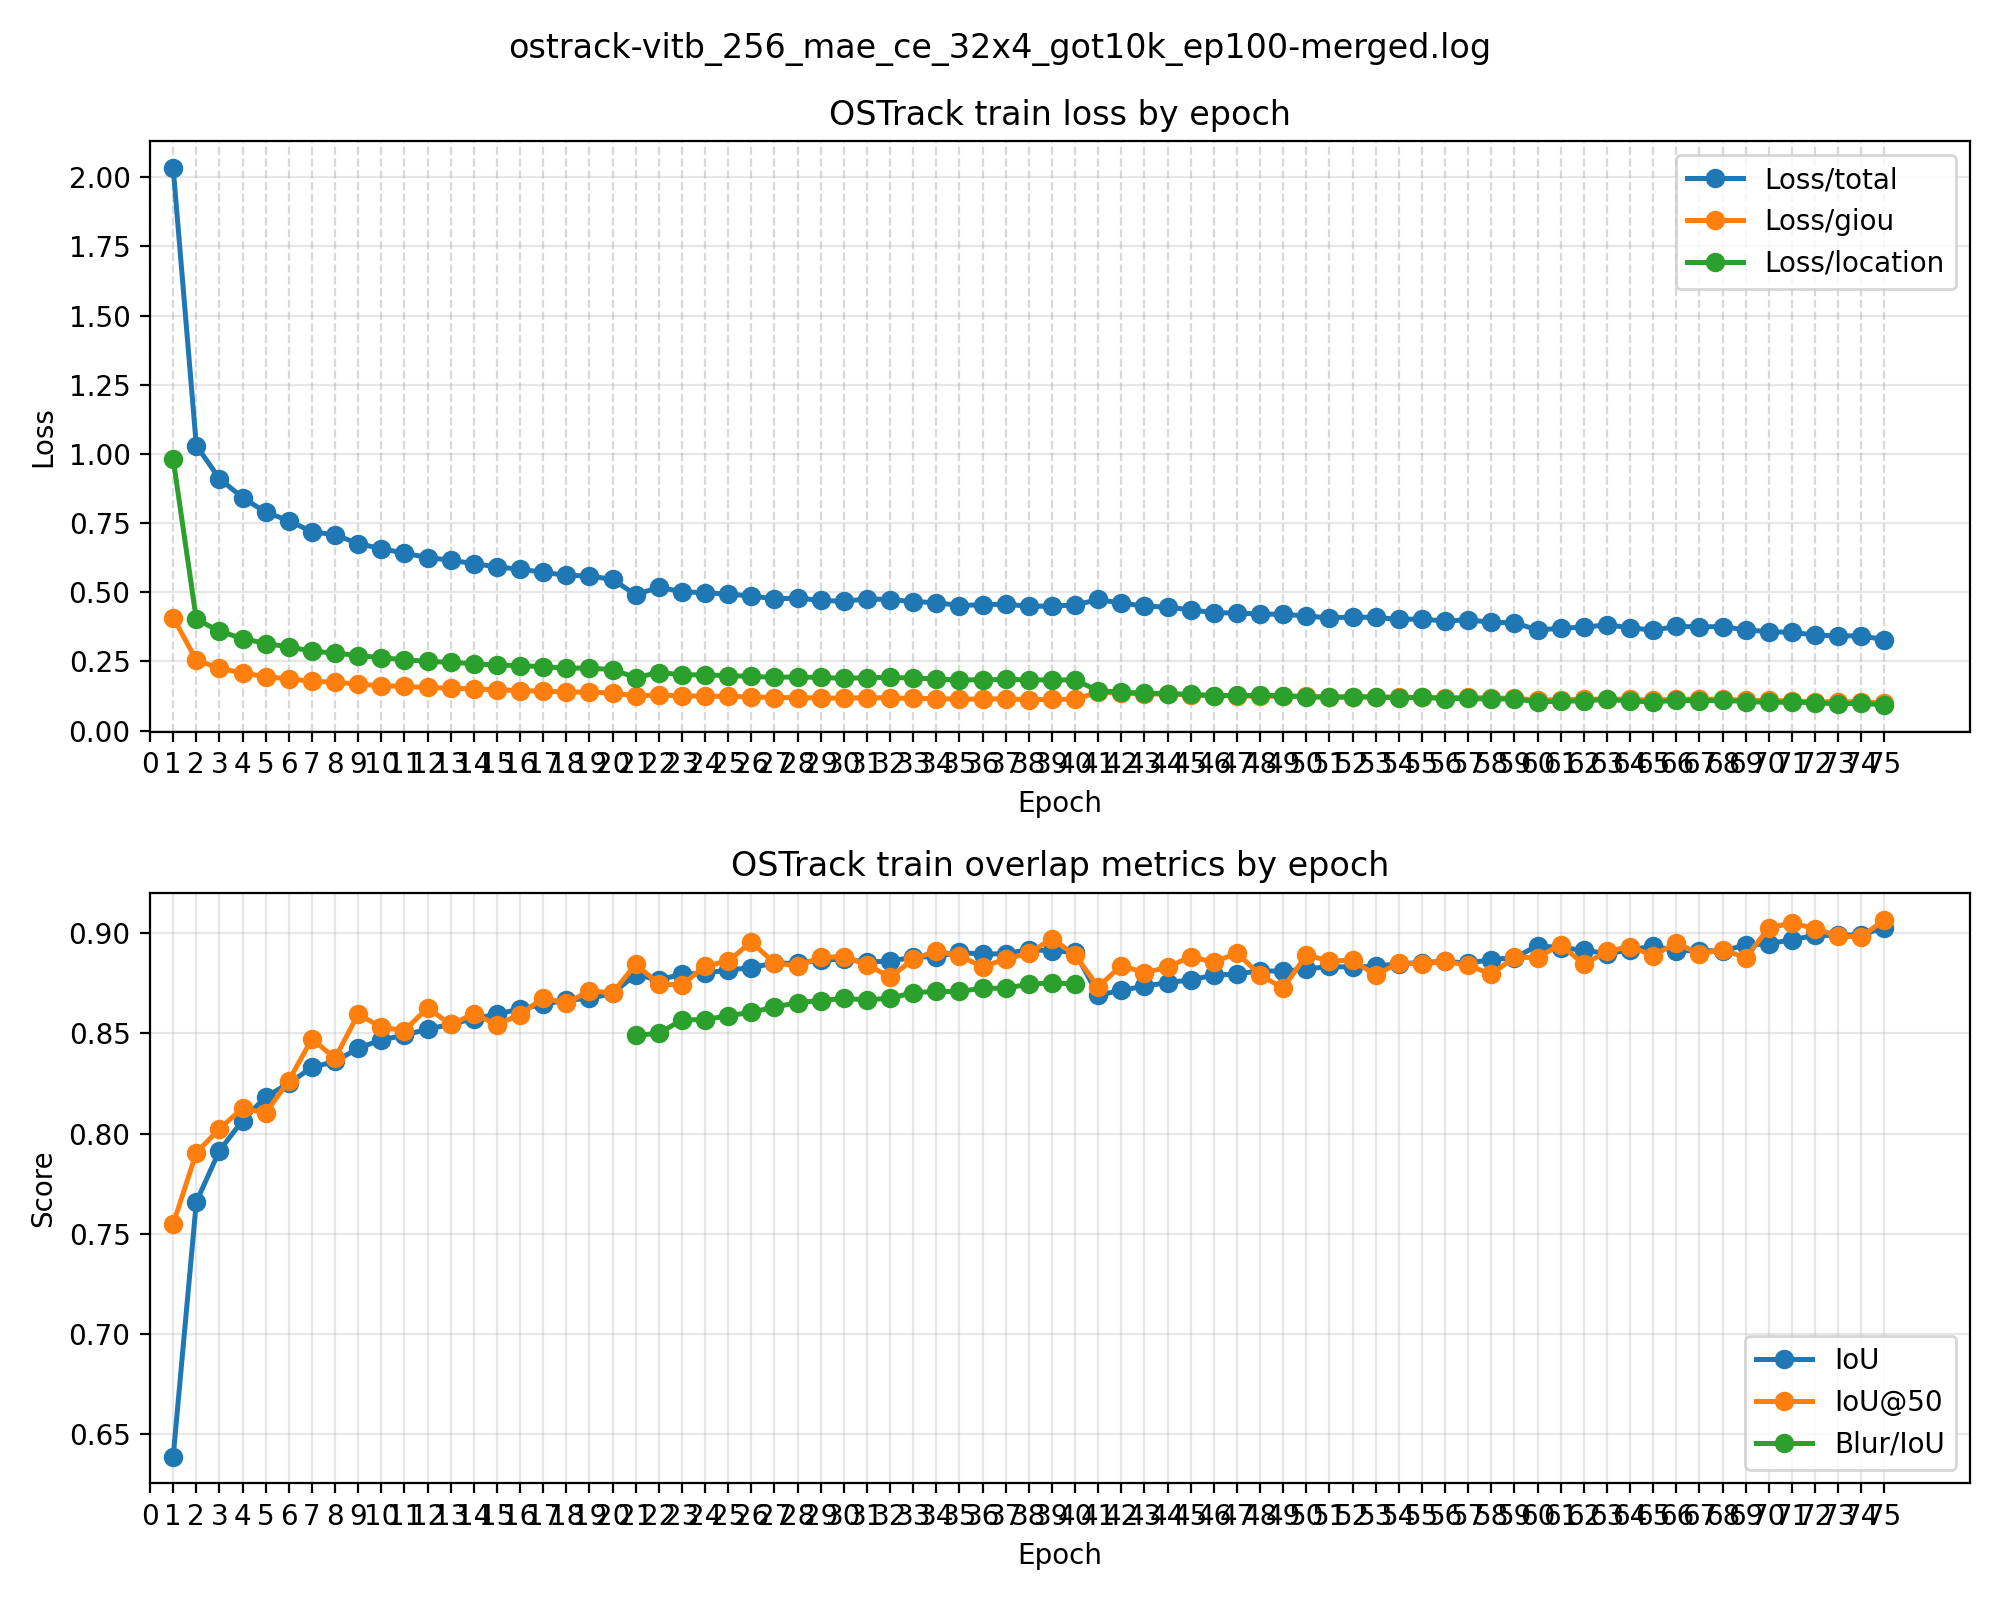
\includegraphics[width=0.9\textwidth]{ostrack-vitb_256_mae_ce_32x4_got10k_ep100_train_epoch_metrics.png}
        \caption{Training loss and overlap metrics over the 75 recorded epochs.}
        \label{fig:train-metrics}
    \end{figure}

    \begin{figure}[htbp]
        \centering
        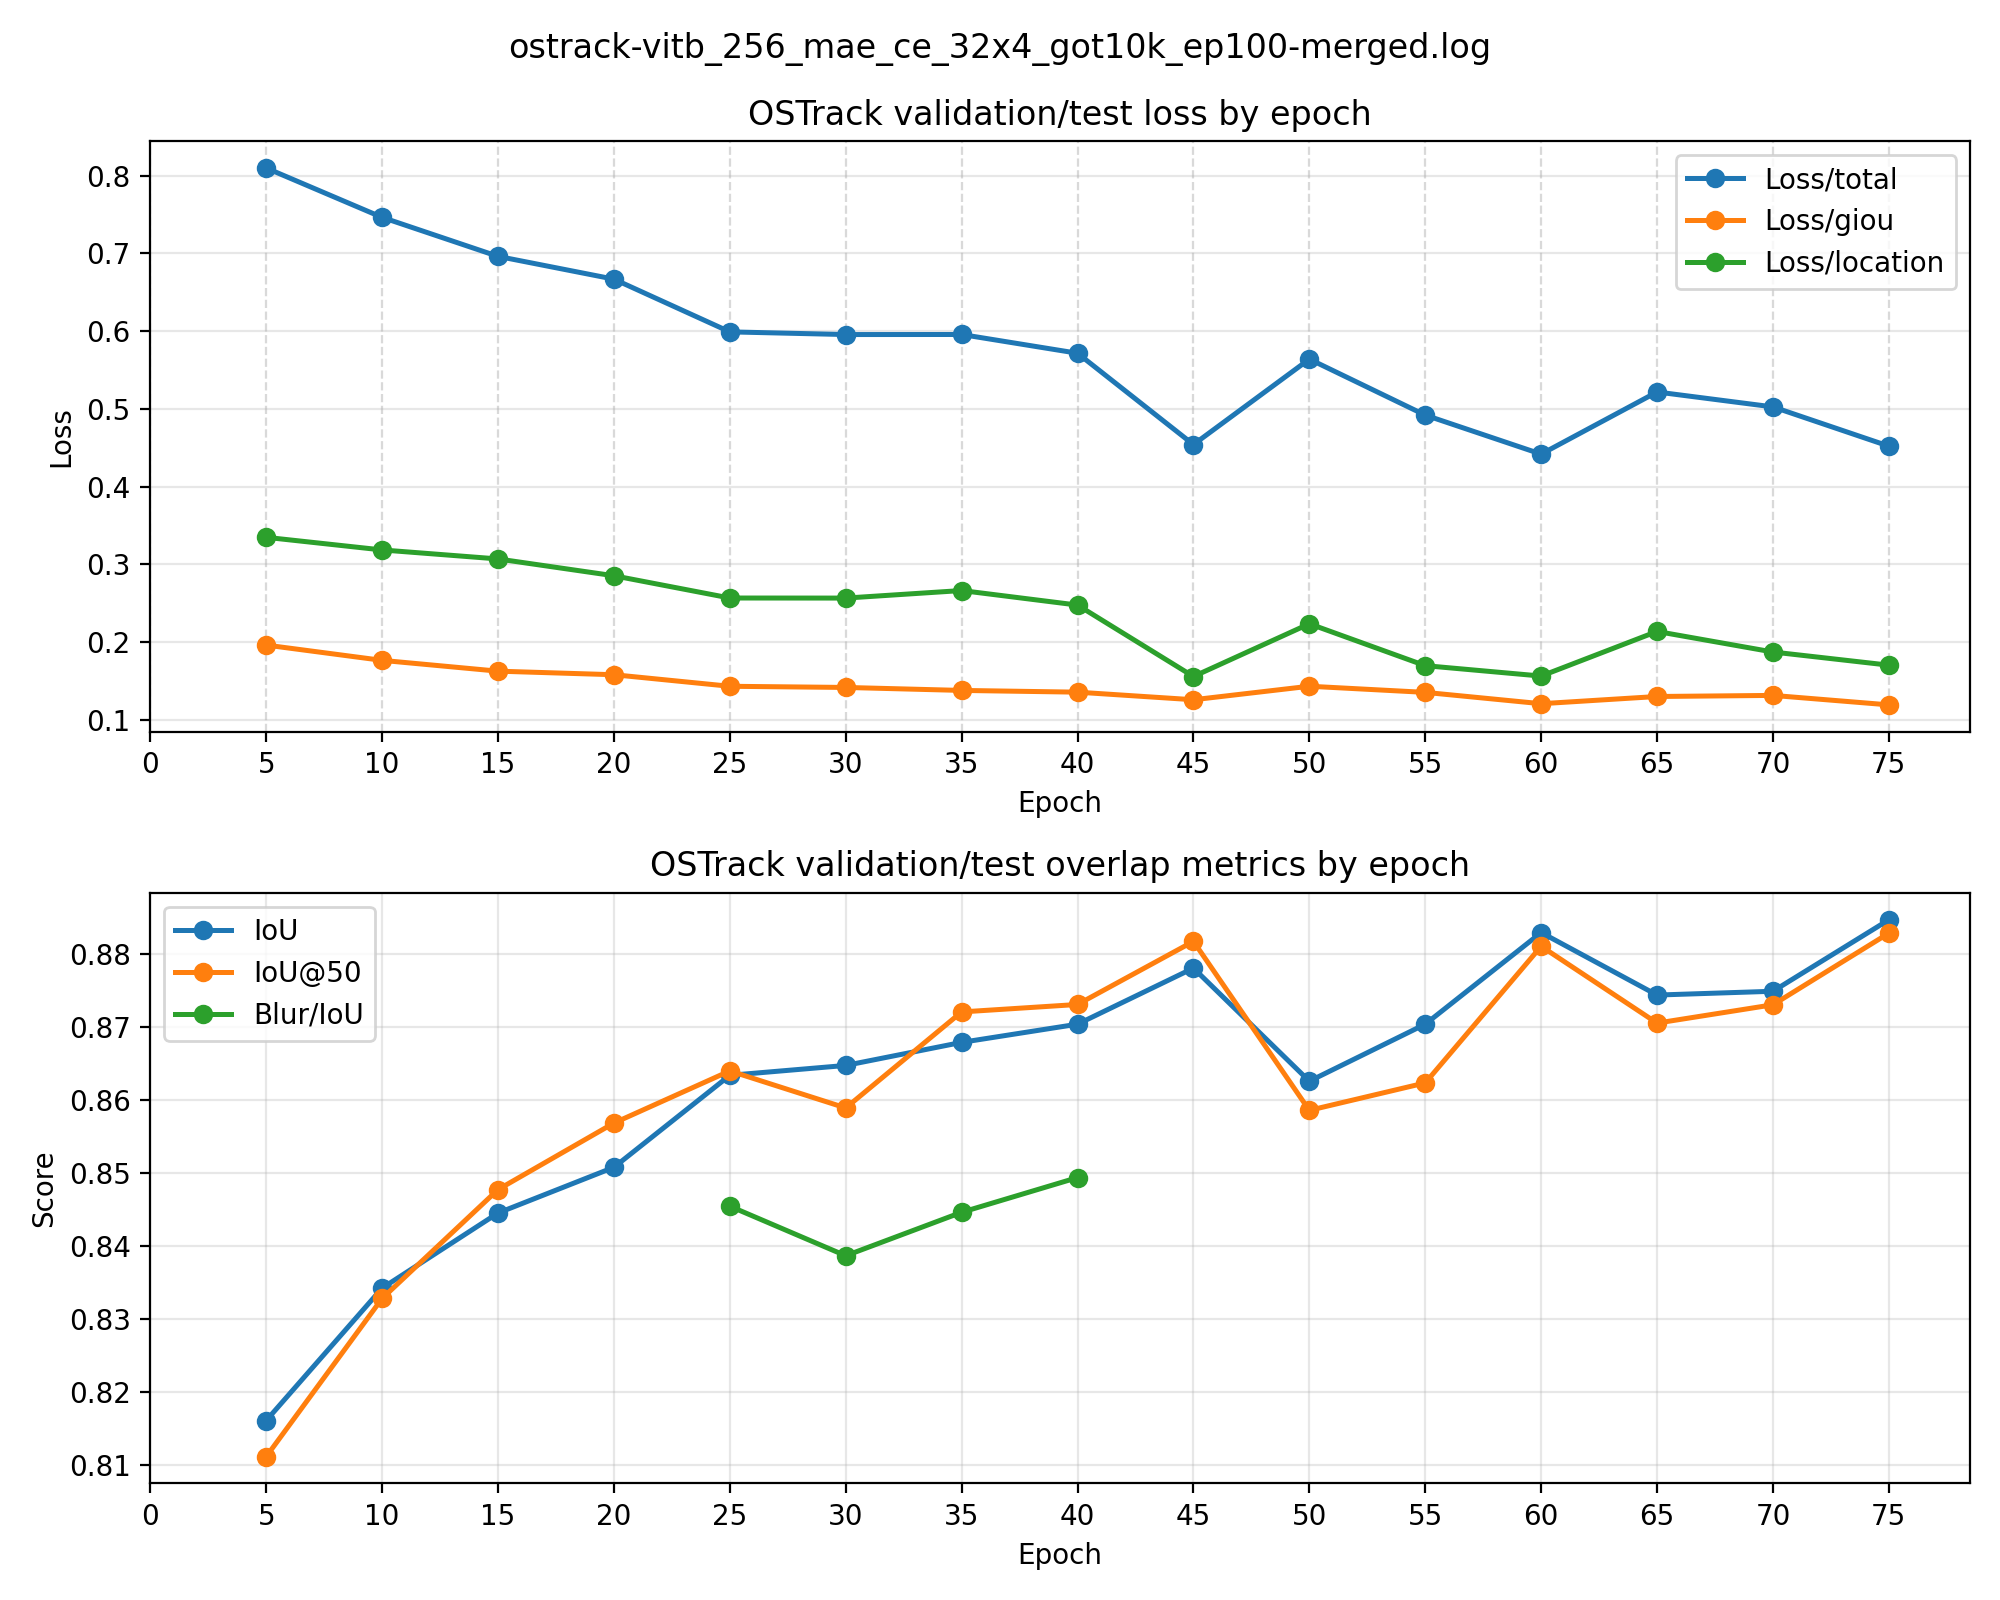
\includegraphics[width=0.9\textwidth]{ostrack-vitb_256_mae_ce_32x4_got10k_ep100_val_test_epoch_metrics.png}
        \caption{Validation loss and overlap metrics recorded every five epochs.}
        \label{fig:validation-metrics}
    \end{figure}

    The training curve shows rapid early convergence during the initial warm-up phase , in which the model is trained with standard ground-truth-centered crops. In this period, the total training loss decreases sharply from 2.033 to 0.547, while the training IoU climbs to approximately 0.870.

    Between epochs 21 and 40, template blurring was introduced to the training pipeline. During this phase, the standard training IoU remained stable and high. More importantly, the model's performance on specifically corrupted templates, tracked via the separate \texttt{Blur/IoU} metric, steadily improved from 0.849 at epoch 21 to a peak of 0.875 at epoch 39. This upward trend indicates that the network successfully adapted to the degraded initial template, forcing it to rely more heavily on the recurrent memory state to maintain accurate localization.

    At epoch 41, template blurring was disabled, and the training pipeline transitioned to the inference-like dynamic
    rollout setting. This shift intentionally introduced a significantly harder optimization objective, as the model was now
    forced to handle its own prediction drift across frames. This increased difficulty is immediately visible in the graphs:
    the GIoU loss spikes from 0.114 to 0.139, and the training IoU drops from 0.891 to 0.869. However, the training metrics recovered in subsequent epochs. A scheduled learning rate decay at epoch 60 resulted in a further, immediate reduction in training loss and a corresponding jump in training accuracy.
    The validation metrics (Figure~\ref{fig:validation-metrics}) support the same interpretation. The validation loss reached its lowest point of 0.442 at
    epoch 60. Although the internal validation IoU continued to rise slightly in later epochs (reaching 0.885 at epoch 75).
    the epoch-60 checkpoint exhibited the best overall validation loss profile.
    For this reason, the epoch-60 checkpoint was selected for the official GOT-10k test evaluation reported in Table~\ref{tab:got10k-results}.


    Overall, the training dynamics show that the model first learns stable localization under clean conditions, then adapts to corrupted-template training, and finally becomes robust to inference-like dynamic cropping.


    \section{Limitations}\label{limitations}

    The most important limitation is the lack of a full ablation study. Because multiple
    changes were introduced, it is not possible to isolate the exact effect of each
    component from the final table alone. For example, the gain over OSTrack-256 + CE may
    come from memory tokens, dynamic cropping, candidate elimination interactions, training
    differences, template blurring, auxiliary losses, or a combination of these factors.

    The second limitation is that the memory mechanism was evaluated mainly on the standard
    metrics. It may be more useful to analyze specific sequence attributes such as
    occlusion, deformation, or long-term appearance change. If memory helps only in certain
    cases, the average score may hide this benefit.

    The third limitation is that memory loss heads were not fully optimized. The balance
    between the main loss and memory loss is difficult and likely important. A scheduled
    memory loss or a warm-up phase may be more stable than applying the full auxiliary loss
    from the beginning.


    \section{Future work}\label{future-work}

    Future work should begin with ablation experiments. The first ablation should compare
    baseline OSTrack, OSTrack with sequence training but no memory, MemOSTrack with static
    ground-truth-centered crops, and MemOSTrack with dynamic crops. This would separate the
    effects of memory and cropping.

    The second ablation should compare memory update mechanisms. A single temporal GRU, the
    current two-stage GRU, and the three-way softmax gated update should be tested under the
    same training conditions. This would reveal whether the layer-wise recurrent connection
    is helpful.

    The third ablation should vary the memory supervision strategy. Possible variants
    include no memory head, memory head after selected layers only, scheduled memory loss,
    and different values of \texttt{lambda\_mem}. Template blurring should also be varied by blur
    strength and probability.

    Finally, the model should be evaluated on sequences where memory is expected to matter:
    long occlusions, viewpoint changes, and gradual appearance changes. If memory helps only
    on a subset of videos, attribute-level analysis may reveal benefits that average metrics
    hide.

    \chapter*{Conclusion}
    \addcontentsline{toc}{chapter}{Conclusion}

    This thesis investigated the integration of recurrent memory tokens into OSTrack. The proposed MemOSTrack model extends the original one-stream transformer tracker with memory tokens updated through ViT and a two-stage GRU update mechanism. The design is intended to provide both temporal continuity and layer-wise memory refinement.

    To effectively train this recurrent architecture, the standard training pipeline was substantially restructured. The original independent pair-based sampling was replaced with sequence-based sampling and inference-like dynamic search cropping, allowing the memory state to evolve over ordered video frames. By generating subsequent search crops from the model's own predictions rather than ground-truth annotations, the training conditions were brought closer to real-world inference, forcing the model to learn how to recover from tracking drift.

    Because a strong baseline tracker can easily bypass newly added modules, explicit and implicit supervision strategies were explored to ensure the memory tokens were actively utilized. Auxiliary memory loss heads were designed to force the memory tokens to encode discriminative spatial features. Concurrently, template blurring was introduced as a regularization technique to reduce the network's over-reliance on the clean initial template, thereby encouraging the extraction of temporal cues from the memory stream.

    In experimental evaluations on the GOT-10k benchmark, the final MemOSTrack-256 + CE model achieved an AO of 0.729, an SR0.50 of 0.823, and an SR0.75 of 0.693. These results demonstrate a clear improvement over the reported same-resolution OSTrack-256 + CE baseline, validating the benefits of the proposed memory mechanism and dynamic training strategy. However, because these modifications were evaluated jointly, future ablation studies are required to determine the individual contributions of the memory tokens, the GRU mechanism, and the dynamic training pipeline to the overall performance gain.

    While Single-Object Tracking (SOT) served as a rigorous and highly useful test framework with established datasets and baselines for this research, the core contributions of this work are not strictly limited to tracking. The proposed integration of recurrent memory tokens, layer-wise GRU updates, and dynamic sequence training provides a robust foundation that could be adapted for broader video processing tasks requiring efficient, long-term temporal modeling in Vision Transformers.

    \clearpage
    \chapter*{References}
    \addcontentsline{toc}{chapter}{References}

    [1] D. Comaniciu, V. Ramesh, and P. Meer, `Real-Time Tracking of Non-Rigid Objects
    Using Mean Shift,' CVPR, 2000.

    [2] B. D. Lucas and T. Kanade, `An Iterative Image Registration Technique with an
    Application to Stereo Vision,' IJCAI, 1981.

    [3] M. Isard and A. Blake, `CONDENSATION - Conditional Density Propagation for Visual
    Tracking,' International Journal of Computer Vision, 1998.

    [4] I. Matthews, T. Ishikawa, and S. Baker, `The Template Update Problem,' IEEE
    Transactions on Pattern Analysis and Machine Intelligence, 2004.

    [5] D. S. Bolme, J. R. Beveridge, B. A. Draper, and Y. M. Lui, `Visual Object Tracking
    using Adaptive Correlation Filters,' CVPR, 2010.

    [6] J. F. Henriques, R. Caseiro, P. Martins, and J. Batista, `Exploiting the Circulant
    Structure of Tracking-by-Detection with Kernels,' ECCV, 2012.

    [7] J. F. Henriques, R. Caseiro, P. Martins, and J. Batista, `High-Speed Tracking with
    Kernelized Correlation Filters,' IEEE Transactions on Pattern Analysis and Machine
    Intelligence, 2015.

    [8] M. Danelljan, G. Hager, F. Shahbaz Khan, and M. Felsberg, `Accurate Scale
    Estimation for Robust Visual Tracking,' BMVC, 2014.

    [9] M. Danelljan, G. Bhat, F. Shahbaz Khan, and M. Felsberg, `ECO: Efficient
    Convolution Operators for Tracking,' CVPR, 2017.

    [10] L. Bertinetto, J. Valmadre, J. F. Henriques, A. Vedaldi, and P. H. S. Torr,
    `Fully-Convolutional Siamese Networks for Object Tracking,' ECCV Workshops, 2016.

    [11] B. Li, J. Yan, W. Wu, Z. Zhu, and X. Hu, `High Performance Visual Tracking with
    Siamese Region Proposal Network,' CVPR, 2018.

    [12] B. Yan, H. Peng, J. Fu, D. Wang, and H. Lu, `Learning Spatio-Temporal Transformer
    for Visual Tracking,' ICCV, 2021.

    [13] B. Ye, H. Chang, B. Ma, S. Shan, and X. Chen, `Joint Feature Learning and
    Relation Modeling for Tracking: A One-Stream Framework,' ECCV, 2022.

    [14] V. Borsuk, R. Vei, O. Kupyn, T. Martyniuk, I. Krashenyi, and J. Matas, `FEAR:
    Fast, Efficient, Accurate and Robust Visual Tracker,' ECCV, 2022.

    [15] G. Bhat, M. Danelljan, L. Van Gool, and R. Timofte, `Learning Discriminative
    Model Prediction for Tracking,' ICCV, 2019.

    [16] J. Shi and C. Tomasi, “Good Features to Track,” Proceedings of the IEEE Conference on Computer Vision and Pattern Recognition, pp. 593–600, 1994.

    [17] L. Huang, X. Zhao, and K. Huang, `GOT-10k: A Large High-Diversity Benchmark for
    Generic Object Tracking in the Wild,' IEEE Transactions on Pattern Analysis and Machine
    Intelligence, 2021.

    [18] A. Vaswani et al., `Attention Is All You Need,' NeurIPS, 2017.

    [19] A. Dosovitskiy et al., `An Image is Worth 16x16 Words: Transformers for Image
    Recognition at Scale,' ICLR, 2021.

    [20] K. Cho et al., `Learning Phrase Representations using RNN Encoder-Decoder for
    Statistical Machine Translation,' EMNLP, 2014.

    [21] K. He, X. Chen, S. Xie, Y. Li, P. Dollar, and R. Girshick, `Masked Autoencoders
    Are Scalable Vision Learners,' CVPR, 2022.

    [22] A. Zhang, Z. C. Lipton, M. Li, and A. J. Smola, `Vision Transformer.svg,'
    Wikimedia Commons, 2024. Licensed under Creative Commons Attribution-ShareAlike 4.0
    International (CC BY-SA 4.0). Available:
    https://commons.wikimedia.org/wiki/File:Vision\_Transformer.svg


    \chapter*{Abstract}
    \addcontentsline{toc}{chapter}{Abstract}

    \section*{Extending OSTrack with GRU-Based Memory Tokens for Visual Object Tracking}

    This thesis investigates the integration of recurrent memory tokens into OSTrack, a
    one-stream transformer tracker. The proposed MemOSTrack model adds memory tokens to
    the template-search token sequence and updates them with a two-stage GRU mechanism using
    previous-frame and previous-layer memory. The training pipeline was rewritten from
    pair-based sampling to ordered video sequence sampling and further extended with dynamic
    search cropping to better match inference. Auxiliary memory loss heads and template
    blurring were explored to encourage the model to use memory. The final model achieved AO
    0.729, SR0.50 0.823, and SR0.75 0.693. It was higher than the reported same-resolution
    OSTrack-256 + CE baseline, but remained slightly below the stronger reported OSTrack-384 + CE baseline.

    Keywords: visual object tracking, OSTrack, transformer, GRU, memory tokens, dynamic
    cropping

    \chapter*{Summary}
    \addcontentsline{toc}{chapter}{Summary}

    \section*{Extending OSTrack with GRU-Based Memory Tokens for Visual Object Tracking}

    The thesis studies whether a transformer-based tracker can benefit from explicit
    recurrent memory. OSTrack is selected as the baseline because it is a strong one-stream
    tracker that jointly processes template and search tokens. The proposed MemOSTrack
    model inserts memory tokens into this token sequence. A transformer layer first produces
    candidate memory, after which a two-stage GRU update combines the candidate with
    previous-frame memory and previous-layer memory.

    A major part of the work is the training pipeline. The original pair-based sampler was
    not sufficient because recurrent memory needs ordered video frames. Therefore, the
    sampler was rewritten to return causal consecutive search sequences. The final pipeline
    also uses dynamic search cropping, where each next search crop is produced from the
    previous prediction. This makes training closer to real inference.

    The thesis also discusses memory loss heads and template blurring. Memory loss heads
    were introduced to prevent the model from ignoring memory tokens. Template blurring was
    explored to reduce over-reliance on the clean initial template and encourage the use of
    temporal memory.

    The final evaluation shows that MemOSTrack-256 + CE achieved AO 0.729, SR0.50
    0.823, and SR0.75 0.693. These results are higher than the reported OSTrack-256 + CE
    baseline, but lower than the reported OSTrack-384 + CE baseline. The main conclusion is
    that the final MemOSTrack configuration is higher than the reported same-resolution 256 CE setting, but
    does not yet surpass the higher-resolution 384 CE model. Further optimization and
    ablation studies are required to separate the effects of memory, dynamic cropping,
    candidate elimination, and resolution.

    \chapter*{Abbreviations}
    \addcontentsline{toc}{chapter}{Abbreviations}

    \begin{longtable}[]{@{}
            >{\raggedright\arraybackslash}p{(\columnwidth - 4\tabcolsep) * \real{0.1525}}
            >{\raggedright\arraybackslash}p{(\columnwidth - 4\tabcolsep) * \real{0.2966}}
            >{\raggedright\arraybackslash}p{(\columnwidth - 4\tabcolsep) * \real{0.5508}}@{}}
        \caption{Abbreviations.}\label{tab:abbreviations} \\
        \toprule\noalign{}
        \begin{minipage}[b]{\linewidth}
            \raggedright
            \textbf{Abbreviation}
        \end{minipage} & \begin{minipage}[b]{\linewidth}
                             \raggedright
                             \textbf{English term}
        \end{minipage} & \begin{minipage}[b]{\linewidth}
                             \raggedright
                             \textbf{Explanation}
        \end{minipage} \\
        \midrule\noalign{}
        \endhead
        \bottomrule\noalign{}
        \endlastfoot
        AO      & Average Overlap                   & Average IoU over evaluated frames                               \\
        BPTT    & Backpropagation Through Time      & Training procedure for recurrent models unrolled over sequences \\
        CE      & Candidate Elimination             & OSTrack efficiency module that removes unlikely tokens          \\
        GOT-10k & Generic Object Tracking benchmark & Large-scale tracking benchmark                                  \\
        GRU     & Gated Recurrent Unit              & Recurrent neural network unit with gates                        \\
        IoU     & Intersection over Union           & Overlap between predicted and ground-truth boxes                \\
        MAE     & Masked Autoencoder                & Self-supervised vision pretraining method                       \\
        SOT     & Single-Object Tracking            & Tracking one specified object through a video                   \\
        SR      & Success Rate                      & Fraction of frames above an IoU threshold                       \\
        ViT     & Vision Transformer                & Transformer model applied to image patches                      \\
    \end{longtable}

\end{document}
